% =====================================================================
%  Manuscript for Journal of Geophysical Research: Planets.
%
%  Title: An Inter-Site Contrast in Lunar Deep Regolith Conductivity
%  from a Per-Site Retrieval Against the Restored Apollo 15 and 17
%  Heat-Flow Experiment Record.
%
%  Build:  pdflatex letter ; bibtex letter ; pdflatex letter ; pdflatex letter
%  Companion supplemental document: appendix.tex.
% =====================================================================
\documentclass[11pt]{article}

\usepackage[a4paper,margin=2.2cm]{geometry}
\usepackage[T1]{fontenc}
\usepackage{lmodern}
\usepackage{microtype}
\usepackage{amsmath,amssymb}
\usepackage{siunitx}
\sisetup{detect-all,per-mode=symbol}
% `year' clashes with the TeX \year count primitive, which makes
% \si{...\per\year} throw "Missing number". Declare an explicit unit.
\DeclareSIUnit{\year}{yr}
\usepackage{graphicx}
\usepackage{booktabs}
\usepackage{caption}
\captionsetup{font=small,labelfont=bf,labelsep=period}
\usepackage[hidelinks,colorlinks=true,linkcolor=blue!50!black,
            citecolor=blue!50!black,urlcolor=blue!60!black]{hyperref}
\usepackage{xcolor}
\usepackage[round,authoryear]{natbib}
\bibliographystyle{plainnat}
\setlength{\bibsep}{2pt}
\renewcommand{\arraystretch}{1.15}

% --- JGR review formatting: continuous line numbers in the left margin -------
% AGU/JGR submissions are reviewed with line numbers; \linenumbers (below,
% after \begin{document}) turns them on. mathlines also numbers display maths.
\usepackage[mathlines]{lineno}

% --- Float placement: keep figures near their references ----------------------
\usepackage{placeins}             % \FloatBarrier
\renewcommand{\topfraction}{0.95}
\renewcommand{\bottomfraction}{0.85}
\renewcommand{\textfraction}{0.05}
\renewcommand{\floatpagefraction}{0.85}
\setcounter{topnumber}{2}
\setcounter{bottomnumber}{2}
\setcounter{totalnumber}{4}

% --- Tighten whitespace around floats (LaTeX defaults are very generous) -----
\setlength{\floatsep}{6pt plus 2pt minus 2pt}
\setlength{\textfloatsep}{8pt plus 2pt minus 4pt}
\setlength{\intextsep}{6pt plus 2pt minus 2pt}
\setlength{\abovecaptionskip}{4pt}
\setlength{\belowcaptionskip}{2pt}

% --- Tighten equation vertical spacing ----------------------------------------
\setlength{\abovedisplayskip}{6pt plus 2pt minus 2pt}
\setlength{\belowdisplayskip}{6pt plus 2pt minus 2pt}
\setlength{\abovedisplayshortskip}{3pt plus 1pt}
\setlength{\belowdisplayshortskip}{3pt plus 1pt}

% --- Tighten section/paragraph heading spacing --------------------------------
\usepackage{titlesec}
\titlespacing*{\section}{0pt}{10pt plus 2pt minus 2pt}{4pt plus 1pt}
\titlespacing*{\subsection}{0pt}{8pt plus 2pt minus 2pt}{3pt plus 1pt}
\titlespacing*{\paragraph}{0pt}{5pt plus 1pt minus 1pt}{1em}

% --- Lightweight \plainlanguagesummary so the layout matches GRL ----
% (Remove this environment when switching to the AGU class.)
\newenvironment{plainlanguagesummary}{%
  \par\medskip\noindent\textbf{Plain Language Summary.}\itshape\small}{\par\medskip}

% --- Convenience macros --------------------------------------------------
\newcommand{\Hayne}{Hayne et al.\ (\citeyear{hayne2017})}
\newcommand{\Vas}{Vasavada \emph{et~al.} (\citeyear{vasavada2012})}
\newcommand{\dT}{\Delta T}
\newcommand{\zborestem}{80\,\si{\centi\meter}}

\title{\bfseries Estimates of Lunar Regolith Thermal Conductivity $K_d$ at Respective Apollo 15 and 17 Heat-Flow Boreholes}

\author{R.~P.~Gregorio\thanks{Independent researcher.
Correspondence to: \texttt{rp3gregorio@gmail.com}.}}

\date{\today}

\begin{document}
\linenumbers
\maketitle

% =====================================================================
\begin{abstract}
\noindent
Apollo 15 and 17 are the only places on the Moon where
deep-regolith temperatures have been measured in situ; their two
Heat-Flow Experiment (HFE) boreholes, with sensors reaching
139 cm (A15) and 234 cm (A17), are the sole direct constraint
on the deep-regolith thermal conductivity $K_d$.
Published parameterizations \citep{hayne2017,martinez2021} are
calibrated globally against orbital Diviner brightness
temperatures, without sub-surface validation. We retrieve $K_d$ at each borehole from the restored
1971--1977 record \citep{nagihara2018} by sweeping $K_d$ against
the deep-sensor RMSE under the \citet{hayne2017} form, with
borestem-contaminated shallow sensors excluded \emph{a priori}.
Conditional on the canonical basal heat flux $Q_b$, the
retrieval yields
$K_{d,\mathrm{A15}}^{*}=4.86^{+1.12}_{-0.54}$ and
$K_{d,\mathrm{A17}}^{*}=11.23^{+8.12}_{-0.77}$
mW m$^{-1}$ K$^{-1}$ ($1\sigma$ non-parametric bootstrap),
reducing the deep-sensor RMSE from 1.37 and 2.96 K under the
published global $K_d=3.4$ to 0.91 and 0.30 K. The
\citet{martinez2021} $K(T,\rho)$ forward reproduces A15 within
1.1 K but underpredicts A17 by 2.5 K; a per-site Mart{\'\i}nez
retrieval requires $\rho_d\!\approx\!3300$ kg m$^{-3}$ at A17
(denser than solid lunar basalt), so the published Mart{\'\i}nez
density term cannot reproduce the A17 deep gradient at canonical
$Q_b$. A15 sits within porosity and orbital benchmarks; A17 is
admissible at the upper porosity and basaltic-composition edges
and rescales to $\sim$7--8 mW m$^{-1}$ K$^{-1}$ under the
\citet{saito2007,nagihara2018} reanalyzed $Q_b$. A17 remains the
more conductive site in every admissible case; the factor-of-two
contrast is marginally significant ($p\approx 0.05$) but robust
in sign. The per-site $K_d^{*}$ values supply the deep $T(z)$
boundary condition needed by sub-surface RTM retrievals and an
in-situ reference for future global conductivity models.
\end{abstract}

\begin{plainlanguagesummary}
The Moon's interior is insulated from the daily surface heating
by the compacted regolith (broken rock and dust) in roughly the
top meter. The numbers describing that insulation come from
formulas fit to satellite measurements of the lunar surface
temperature, not to any direct sub-surface data. Sub-surface
temperatures were measured at only two locations, by
thermometers emplaced more than two meters deep by the Apollo 15
and 17 astronauts in 1971--1972, and the complete records were
recently recovered from the original mission tapes. We use those
two records to determine, separately at each borehole, the
regolith conductivity at depths below about 30 cm, where the
daily surface temperature swing has died away and the
conductivity has settled to a steady value. The Hayne (2017)
global value misses the deep temperatures by about 1.4 K at
Apollo 15 and 3.0 K at Apollo 17; site-by-site refitting reduces
those errors to $\lesssim$1 K, and the two sites disagree on the
deep conductivity by roughly a factor of two. The site-fit
values provide the deep-temperature input that upcoming lunar
sub-surface mapping missions, such as TSUKIMI, will need to
interpret what their instruments observe through the regolith.
\end{plainlanguagesummary}

\medskip
\noindent\textbf{Key Points}
\begin{itemize}\itemsep2pt
  \item Per-site HFE retrieval gives
        $K_d^{\mathrm{A15}}=4.86^{+1.12}_{-0.54}$ and
        $K_d^{\mathrm{A17}}=11.23^{+8.12}_{-0.77}$
        mW m$^{-1}$ K$^{-1}$ ($1\sigma$ bootstrap),
        a factor-of-two inter-site contrast.
  \item Per-site fit cuts the deep-sensor RMSE from 1.4 and 3.0 K
        (Hayne global) to 0.9 and 0.3 K, conditional on $Q_b$.
  \item Site-fit $K_d^{*}$ values supply the deep-$T(z)$ boundary
        condition for sub-surface RTM modelling (TSUKIMI mission).
\end{itemize}

% =====================================================================
\section{Introduction}\label{sec:intro}

Lunar sub-surface thermal modelling presently relies on globally
averaged conductivity parameterizations. We use the term
\emph{deep regolith} throughout to mean depths
$z\gtrsim 30$ cm, where the daily surface heat wave has damped
to undetectable amplitude and the conductivity in both standard
parameterizations has effectively reached its depth-independent
asymptote $K_d$; the daily skin itself spans $\lesssim 10$ cm.
The deep-regolith conductivity is supplied by formulations
calibrated against orbital Diviner brightness temperatures: the
smooth-exponential $K(T,z)$ of \citet{hayne2017}, in which a
single deep-regolith asymptote $K_d$ is fit to a global average
and applied moon-wide, and the temperature- and density-dependent
$K(T,\rho)$ of \citet{martinez2021}, which extends the same
functional family with additional physical content but is itself
calibrated globally and applied uniformly. Both parameterizations
probe only the diurnal
skin. The extent to which the resulting global $K_d$ represents
any individual landing site, and the magnitude of any site-to-site
departure, cannot be determined from orbital data alone.

Direct in-situ data exist only from the Apollo Heat-Flow
Experiment (HFE). At Apollo 15 and 17, fibreglass borestems
emplaced by the astronauts carried thermometers to depths
exceeding two meters
\citep{langseth1972,langseth1976}; these two boreholes remain the
only lunar locations at which a sub-surface temperature profile
has been measured (Fig.~\ref{fig:intro-probe}). The restored
1971--1977 HFE record \citep{nagihara2018} provides the data used
here. Each borehole also carries a published basal heat flux
\citep{langseth1976,nagihara2018} which, together with the local
$K_d$, sets the deep temperature gradient. The site-specific
inputs (latitudes, albedos, emissivities, basal fluxes) are
collected with their original sources in Table~\ref{tab:params}.

We retrieve $K_d$ separately at each site by holding the
\citet{hayne2017} functional form fixed and sweeping $K_d$ alone
against the deep-sensor RMSE. The retrieval is placed in context
by two additional forward evaluations against the same deep-sensor
set: the \citet{hayne2017} form at its published global $K_d$, and
the \citet{martinez2021} $K(T,\rho)$ model at its published
coefficients (Table~\ref{tab:headline}). Neither published model
is refit here, so the \citet{martinez2021} comparison quantifies
the performance of the published global $K(T,\rho)$ at each Apollo
site without per-site freedom. A full per-site retrieval under the
\citet{martinez2021} form requires a different choice of free
parameter from $K_d$ and is deferred to a follow-on study
(\S\ref{sec:disc-prior}).

The per-site $K_d^{*}$ values matter for any sub-surface
radiative-transfer (RTM) retrieval that observes the Moon at
wavelengths penetrating below the diurnal skin: future microwave,
terahertz, and infrared sub-surface sounders all need a deep
temperature column $T(z)$ as a forward-model boundary condition
that orbital instruments cannot measure directly. One concrete
example is the upcoming TSUKIMI mission (Lunar Terahertz Surveyor
for Kilometer-scale Mapping, \citealp{tsukimi2022}), whose
terahertz radiometer will probe depths comparable to the Apollo
HFE sensors and so depends explicitly on $K_d$. Because the
emission-weighting kernel of any such instrument reaches depths
at which the conductivity has approached its asymptote $K_d$, the
retrieved $T(z)$ depends on $K_d$ and not only on the shallow-skin
$K_s$; a factor-of-two error in $K_d$ propagates through the deep
temperature profile and into any retrieval that uses it. The
values reported here, evaluated in the \citet{hayne2017} thermal
column, supply that boundary condition from the only in-situ data
available.\label{sec:intro-tsukimi}

The retrieval is driven by an ephemeris-accurate solar-forcing
chain (JPL DE440 lunar and solar positions accessed through SPICE;
\citealp{acton1996,acton2018}), which eliminates the $\sim$1
lunar-hour drift inherent in sinusoidal local-solar-time
approximations and is required by the phase-folded
diurnal-amplitude profile underlying the borestem cut
(\S\ref{sec:results-amp}). The remaining sections present the
data and methods (\S\ref{sec:methods}), the per-site retrieval
with the headline RMSE table (\S\ref{sec:results}), the
interpretation with its uncertainty limits
(\S\ref{sec:discussion}), and the conclusions.

\begin{figure}[htbp]
\centering

\includegraphics[width=\linewidth]{figures/fig_intro_probe.pdf}
\caption{Apollo HFE measurement geometry and the two published
$K(z)$ forms tested. \textbf{(a)} Probe schematic showing the
fibreglass borestem and thermometer placements (Apollo~15 Probe-1).
Coral band: borestem-excluded zone ($z<80$ cm); teal markers:
deep sensors used in the retrieval. \textbf{(b)} Thermal
conductivity profiles $K(z)$ at $T=250$ K: \citet{hayne2017}
smooth-exponential form at $K_d^{\mathrm{publ.}}=3.4$
mW m$^{-1}$ K$^{-1}$ (solid teal); \citet{martinez2021}
$K(T,\rho)$ at published coefficients (dashed red). Both use
the same Hayne-form $\rho(z)$.}
\label{fig:intro-probe}
\end{figure}

\begin{figure}[htbp]
\centering
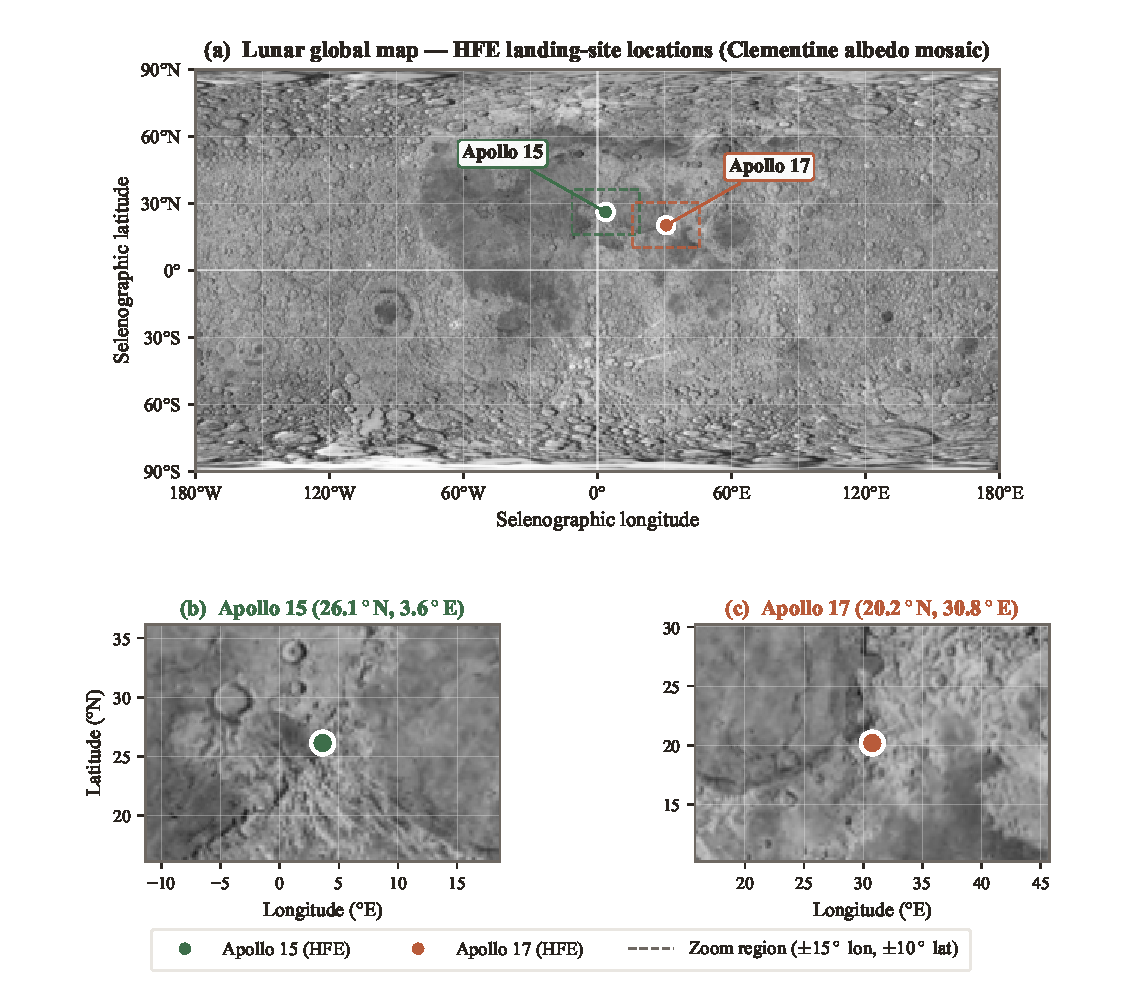
\includegraphics[width=\linewidth]{figures/fig_context_map.pdf}
\caption{Apollo Heat-Flow Experiment landing-site context on the
Clementine global albedo mosaic (USGS/NASA, public domain).
\textbf{(a)} Global equirectangular map showing the two HFE
boreholes; dashed coloured rectangles mark the zoom regions of
panels (b) and (c). \textbf{(b)} Apollo 15 regional zoom
($\pm 15^\circ$ longitude, $\pm 10^\circ$ latitude), Imbrium--
Apennine boundary, mare/highland margin. \textbf{(c)} Apollo 17
regional zoom, basaltic embayment of Mare Serenitatis at the
Taurus--Littrow highlands edge
\citep{korotev2005,wieczorek2006,crawford2015}. Borehole
coordinates from the ALSEP gazetteer.}
\label{fig:context-map}
\end{figure}

% =====================================================================
\section{Data and Methods}\label{sec:methods}

\subsection{Apollo HFE deep-sensor temperatures}
The retrieval requires one equilibrium temperature $T_\mathrm{eq}$
per sensor. The restored 1971--1977 record \citep{nagihara2018}
provides this quantity once the early portion of each record,
which contains residual transients from drilling and emplacement,
documented mission-operations disturbances \citep{nagihara2018},
and slow instrumental drift, is excluded. For each sensor we
extract automatically the longest trailing segment that is
statistically indistinguishable from a flat steady state and
average within it.

For each sensor, candidate start points covering 55--85\% of the
record (in 13 equally-spaced steps) are evaluated by
ordinary-least-squares linear fit to all temperatures between the
candidate point and the end of the record. The accepted
\emph{stability window} is the earliest candidate for which the
linear-fit slope satisfies
$|d\langle T\rangle/dt|<0.08\,\si{\kelvin\per\year}$
($\approx 2.2\times 10^{-4}\,\si{\kelvin\per\day}$): the longest
tail consistent with thermal equilibrium at this stringency. The
adopted threshold is approximately $4.6\times$ stricter than the
$10^{-3}\,\si{\kelvin\per\day}$ value sometimes used in HFE
analyzes, and was chosen to suppress bias from residual
post-disturbance drift. If no candidate satisfies the criterion,
the last 25\% of the record is used as a fallback. We report the
window-mean equilibrium temperature
$T_\mathrm{eq}=\langle T(z)\rangle_{\Delta t}$ together with its
within-window standard deviation, which serves as the per-sensor
measurement uncertainty in downstream statistics. Sensors with
central depth $z<\zborestem$ (the borestem-contaminated zone;
\S\ref{sec:borestem}) are plotted but excluded from the RMSE.
Figure~\ref{fig:timeline} shows the full per-probe temperature
record at each site, with the documented disturbance intervals
shaded \citep{nagihara2018}, the selected stability windows
marked, and the fitted long-term drift $d\langle T\rangle/dt$
reported per sensor.

The retrieval is insensitive to the precise threshold. Sweeping the
threshold over $0.04$--$\SI{0.16}{\kelvin\per\year}$ (a factor of
four around the adopted value) shifts $K_d^{*}$ by at most
$0.03\,\si{\milli\watt\per\meter\per\kelvin}$ at A15 (0.7\% of
nominal) and $0.11\,\si{\milli\watt\per\meter\per\kelvin}$ at A17
(1.0\%), in both cases an order of magnitude below the
bootstrap $1\sigma$ uncertainty (\S\ref{sec:results-kd}). The
adopted threshold therefore lies within the flat band of the
threshold response.

\begin{figure}[!htbp]
\centering
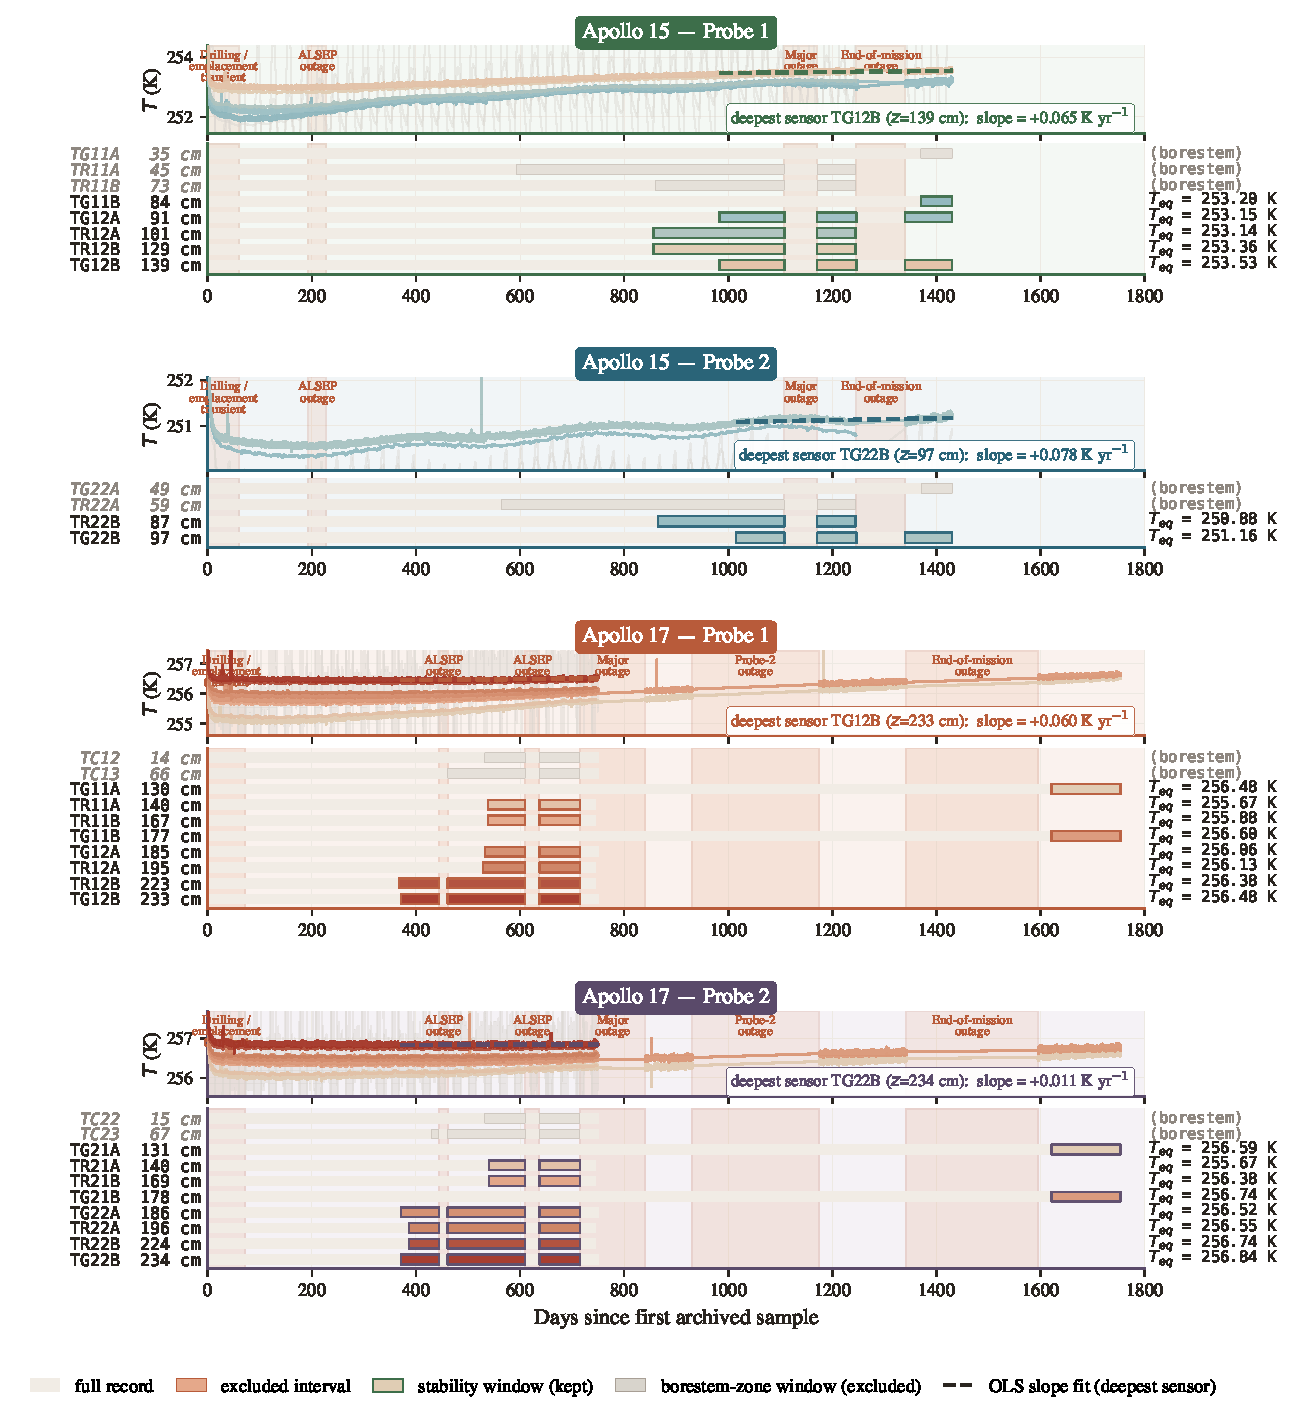
\includegraphics[width=\linewidth]{figures/fig_apollo_timeline.pdf}
\caption{Per-probe stability-window timeline at Apollo~15 and~17
(4 probes). Each probe panel shows, above, the raw HFE traces with
coral bands marking documented data-quality events and the selected
stability windows outlined; and, below, a depth-coded per-sensor
Gantt strip broken at outages. Selection criteria and the role of
the window-mean $T_\mathrm{eq}$ are described in
\S\ref{sec:methods}.}
\label{fig:timeline}
\end{figure}

\subsection{Surface solar geometry and incident insolation}
Each Apollo Unix timestamp is propagated through SPICE
\citep{acton1996,acton2018} using the JPL DE440 planetary
ephemeris and the IAU-defined mean-Earth/polar-axis lunar
body-fixed reference frame, with light-time and stellar-aberration
corrections applied, to obtain the solar zenith angle
$\theta_\odot(t)$ at each site. The Moon has no atmosphere, so
the solar irradiance incident on the local horizontal surface is
\begin{equation}
F_\odot(t) = \max\bigl(0,\ S_0\cos\theta_\odot(t)\bigr),
\label{eq:insolation}
\end{equation}
with $S_0 = 1361\,\si{\watt\per\meter\squared}$ \citep{kopp2011}.

\subsection{1-D solver and \Hayne\ thermophysics}\label{sec:solver}

The depth coordinate $z$ is defined positive downward, with the
regolith surface at $z=0$ and the lower boundary of the modelled
column at $z=z_\mathrm{max}=5$ m. Conservation of energy in
one dimension gives the heat equation
\begin{equation}
\rho(z)\,c_p(T)\,\frac{\partial T}{\partial t}
   = \frac{\partial}{\partial z}\!\Bigl[\,K(T,z)\,\frac{\partial T}{\partial z}\Bigr].
\label{eq:heat}
\end{equation}
At the upper boundary the skin temperature $T_s$ satisfies
radiative balance between absorbed insolation, emitted thermal
radiation, and the conductive flux into the column,
\begin{equation}
(1-A)\,F_\odot(t)\;-\;\varepsilon\sigma T_s^4
\;-\;\bigl(-K\,\partial_z T\bigr)_{\!z=0} \;=\; 0,
\label{eq:bc-top}
\end{equation}
with $\sigma=5.6704\times10^{-8}$ W m$^{-2}$ K$^{-4}$ the
Stefan--Boltzmann constant.
solved iteratively for $T_s$ at each time step. At the lower
boundary a constant geothermal flux is imposed,
\begin{equation}
-K\,\partial_z T\big|_{z_\mathrm{max}} = Q_b.
\label{eq:bc-bot}
\end{equation}
The PDE is discretised on a geometric grid
($\Delta z_0=2$ mm, growth ratio 1.08) and integrated with a
Crank--Nicolson scheme at $\Delta t = 1$ h, with a spin-up of
30 lunations to $\max|\Delta T|<5\times10^{-2}$ K.
The \citet{hayne2017} thermophysical inputs are adopted as given
in Appendix A of the original paper:
\begin{align}
K(T,z) &= \Bigl\{K_s + (K_d-K_s)\bigl[1-e^{-z/H}\bigr]\Bigr\}
         \cdot\Bigl[1 + \chi\bigl(T/T_\mathrm{ref}\bigr)^3\Bigr], \label{eq:K} \\
\rho(z) &= \rho_d - (\rho_d-\rho_s)\,e^{-z/H}, \label{eq:rho}\\
c_p(T)  &= c_0 + c_1 T + c_2 T^2 + c_3 T^3 + c_4 T^4. \label{eq:cp}
\end{align}
Numerical values and sources for every coefficient, together
with the site-specific measured quantities (latitude, albedo,
emissivity, basal heat flux), are listed in
Table~\ref{tab:params}. The basal heat flux reanalyzes of
\citet{saito2007,nagihara2018} are folded into the sensitivity
sweep of \S\ref{sec:results-kd}.

\begin{table}[!htbp]
\centering
\footnotesize
\setlength{\tabcolsep}{4pt}
\renewcommand{\arraystretch}{1.10}
\caption{\textbf{Fixed inputs to the 1-D heat solver.} Three blocks:
(A)~the \citet{hayne2017} conductivity-form coefficients
(eq.~\ref{eq:K}), with $K_d$ the single parameter retrieved in
\S\ref{sec:methods-kd}; (B)~the four published coefficients of the
\citet{martinez2021} $K(T,\rho)$ comparison model (eq.~\ref{eq:K-ms},
forward only in the headline table; see also \S\ref{sec:disc-prior});
(C)~site-specific measured quantities shared by both conductivity
models. The shared $\rho(z)$ uses the Hayne-form profile
(eq.~\ref{eq:rho}); the specific heat is the
\citet{hemingway1973} polynomial
$c_p(T)=c_0+c_1 T+c_2 T^2+c_3 T^3+c_4 T^4$ with
$(c_0,\ldots,c_4)=(-3.61,\,2.74,\,2.36\!\times\!10^{-3},\,
{-1.23}\!\times\!10^{-5},\,8.91\!\times\!10^{-9})$.}
\label{tab:params}
\begin{tabular}{@{} l l l p{0.20\linewidth} p{0.22\linewidth} @{}}
\toprule
Parameter & Symbol & Value & Unit & Source \\
\midrule
\multicolumn{5}{@{}l}{\textit{(A) Hayne et al.\ (2017) smooth-exponential conductivity, all values from \citet{hayne2017} App.~A unless noted}} \\[2pt]
Surface conductivity        & $K_s$              & $7.4\times10^{-4}$  & W\,m$^{-1}$\,K$^{-1}$ &  \\
Deep conductivity (global)  & $K_d$ (publ.)      & $3.4\times10^{-3}$  & W\,m$^{-1}$\,K$^{-1}$ &  \\
Deep conductivity (per-site)& $K_d^{*}$          & \S\ref{sec:results-kd} & W\,m$^{-1}$\,K$^{-1}$ & \textbf{this work} \\
$K(z)$ transition scale     & $H$                & 0.06                & m                     &  \\
Radiative coefficient       & $\chi$             & 2.7                 & ---                   &  \\
Radiative normalisation     & $T_\mathrm{ref}$   & 350                 & K                     &  \\
\midrule
\multicolumn{5}{@{}l}{\textit{(B) Mart\'inez \& Siegler (2021) $K(T,\rho)$ \emph{(forward only)}, coefficients from \citet{martinez2021}}} \\[2pt]
Contact, $\rho$-slope       & $A_1$              & $5.082\times10^{-6}$   & W\,m$^{-1}$\,K$^{-1}$ (kg\,m$^{-3})^{-1}$ &  \\
Contact, intercept          & $A_2$              & $-5.10\times10^{-3}$   & W\,m$^{-1}$\,K$^{-1}$  &  \\
Radiative, $\rho$-slope     & $B_1$              & $2.002\times10^{-13}$  & W\,m$^{-1}$\,K$^{-4}$ (kg\,m$^{-3})^{-1}$ &  \\
Radiative, intercept        & $B_2$              & $-1.953\times10^{-10}$ & W\,m$^{-1}$\,K$^{-4}$  &  \\
\midrule
\multicolumn{5}{@{}l}{\textit{Shared by both conductivity models}} \\[2pt]
Surface bulk density        & $\rho_s$           & 1100                & kg\,m$^{-3}$           & \citet{hayne2017} \\
Deep bulk density           & $\rho_d$           & 1800                & kg\,m$^{-3}$           & \citet{hayne2017} \\
Specific heat               & $c_p(T)$           & polyn.\ (caption)   & J\,kg$^{-1}$\,K$^{-1}$ & \citet{hemingway1973} \\
\midrule
\multicolumn{5}{@{}l}{\textit{(C) Site-specific measured inputs}\quad\textit{(A15\,/\,A17)}} \\[2pt]
Latitude                    & $\phi$             & $26.1^\circ$\,/\,$20.2^\circ$\,N & --- & ALSEP gazetteer \\
Bond albedo                 & $A$                & $0.131$\,/\,$0.137$ & ---                   & \citet{vasavada2012} \\
Broadband emissivity        & $\varepsilon$      & $0.95$              & ---                   & \citet{bandfield2015} \\
Basal heat flux             & $Q_b$              & $21$\,/\,$15$       & mW\,m$^{-2}$          & \citet{langseth1976,nagihara2018} \\
Solar constant              & $S_0$              & $1361$              & W\,m$^{-2}$           & \citet{kopp2011} \\
\bottomrule
\end{tabular}
\end{table}

As an independent comparison we also evaluate the
\citet{martinez2021} regolith conductivity model. Where
\citet{hayne2017} prescribes a depth-dependent envelope through
$K(T,z)=[K_s+(K_d-K_s)(1-e^{-z/H})](1+\chi(T/T_\mathrm{ref})^3)$,
\citet{martinez2021} replaces that envelope with an explicitly
density-dependent two-mechanism decomposition,
\begin{equation}
K(T,\rho) = \underbrace{(A_1\rho + A_2)\,k_\mathrm{am}(T)}_{\text{contact (phonon)}}
          \;+\; \underbrace{(B_1\rho + B_2)\,T^3}_{\text{radiative}}.
\label{eq:K-ms}
\end{equation}
The first term is the contact (phonon) conductivity transmitted
through the network of grain-to-grain contacts; it carries the
temperature dependence of an amorphous solid through the
low-temperature polynomial $k_\mathrm{am}(T)$ of
\citet{martinez2021} and scales linearly with the local bulk
density, reflecting the increased number of grain-to-grain
contacts per unit volume at higher packing. The second term is the
radiative contribution from infrared photon exchange across pore
voids; it scales as $T^3$ (the derivative of the Stefan--Boltzmann
emission with respect to temperature, characteristic of
photon-mediated transport) and is density-modulated with the
opposite physical content, since denser packing reduces the void
fraction available for radiative exchange. The four coefficients
$(A_1,A_2,B_1,B_2)$ are calibrated globally against Diviner
brightness temperatures and are listed in Table~\ref{tab:params}.
The density profile $\rho(z)$ used in this comparison is the same
Hayne-form exponential used in the Hayne column, so the two
models differ in their $K$ formulation alone.

The \citet{martinez2021} formulation has no single $K_d$
analogous to the parameter retrieved under the Hayne form: both
terms in equation~(\ref{eq:K-ms}) vary continuously with depth
through $\rho(z)$ and with temperature through $T(z)$. The
published model contains no free parameter, so its evaluation at
each site yields a single forward prediction
(Table~\ref{tab:headline}). To diagnose, in the discussion
(\S\ref{sec:disc-prior}), whether the published \citet{martinez2021}
form could fit both sites if it were granted one per-site lever
analogous to the Hayne $K_d$, we additionally perform an
alternative retrieval in which the deep asymptote of the
Hayne-form density profile entering equation~(\ref{eq:K-ms}) is
rescaled by a single per-site scalar $\alpha$,
\begin{equation}
\rho_d^{\,\text{site}} \;=\; \alpha\cdot 1800\ \mathrm{kg\,m^{-3}},
\label{eq:alpha}
\end{equation}
with $\rho_s=1100$ kg m$^{-3}$, the e-folding depth $H$, and the
published coefficients $(A_1,A_2,B_1,B_2)$ and $k_\mathrm{am}(T)$
held fixed; $\alpha=1$ recovers the published forward prediction.
The scalar $\alpha$ is our diagnostic construction (the
\citet{martinez2021} model itself is not refit, only re-evaluated
at a per-site density), and its physical interpretation is the
per-site deep bulk density that the published $K(T,\rho)$ would
require to reproduce the in-situ data. The $\alpha$ retrieval is
not part of the headline $K_d$ result; it is interpreted in
\S\ref{sec:disc-prior}.

\subsection{Borestem diagnostic and the deep-sensor
cut}\label{sec:results-amp}\label{sec:borestem}
The deep ($z>\zborestem$) sensor set used in the $K_d$ retrieval
is defined by a physics-based amplitude diagnostic, not by the
residuals it would produce. The amplitude of the diurnal wave
serves as a frequency-domain check independent of the
annual-mean comparison. The per-sensor diurnal amplitude is
computed as the half-range of the local-solar-time-folded
median temperature (Fig.~\ref{fig:amplitude}). Two features are
diagnostic. Above $z=\zborestem$, observed amplitudes exceed
the modelled regolith-attenuation curve by an order of magnitude
or more, the signature of heat conducted along the fibreglass
borestem from the lunar surface, which thermally short-circuits
the upper $\sim\zborestem$ of regolith \citep{nagihara2018}.
Below $\zborestem$, both published $K(z)$ forms predict diurnal
amplitudes $\lesssim 10^{-7}$ K ($\sim$18 e-foldings of the
diurnal skin depth $\delta\sim 3$--5 cm), two to three orders of
magnitude below the 0.05--0.2 K digitisation noise floor of the
restored record. Deep-sensor amplitudes therefore do not
constrain the thermal diffusivity $\kappa = K/(\rho c_p)$ at the
in-situ scale; the Hayne and \citet{martinez2021} attenuation
curves plotted in Figure~\ref{fig:amplitude} agree to within
$\sim$10\% in skin depth and overlap visually below the noise
floor, both indicating ``deep $=$ unresolved''. The shallow-sensor
amplitude excess, evaluated against a prediction that depends
only on $K(T,z)$, $\rho(z)$, and $c_p(T)$, defines the deep
($z>\zborestem$) validation set used in the retrieval.

\begin{figure}[!htbp]
\centering
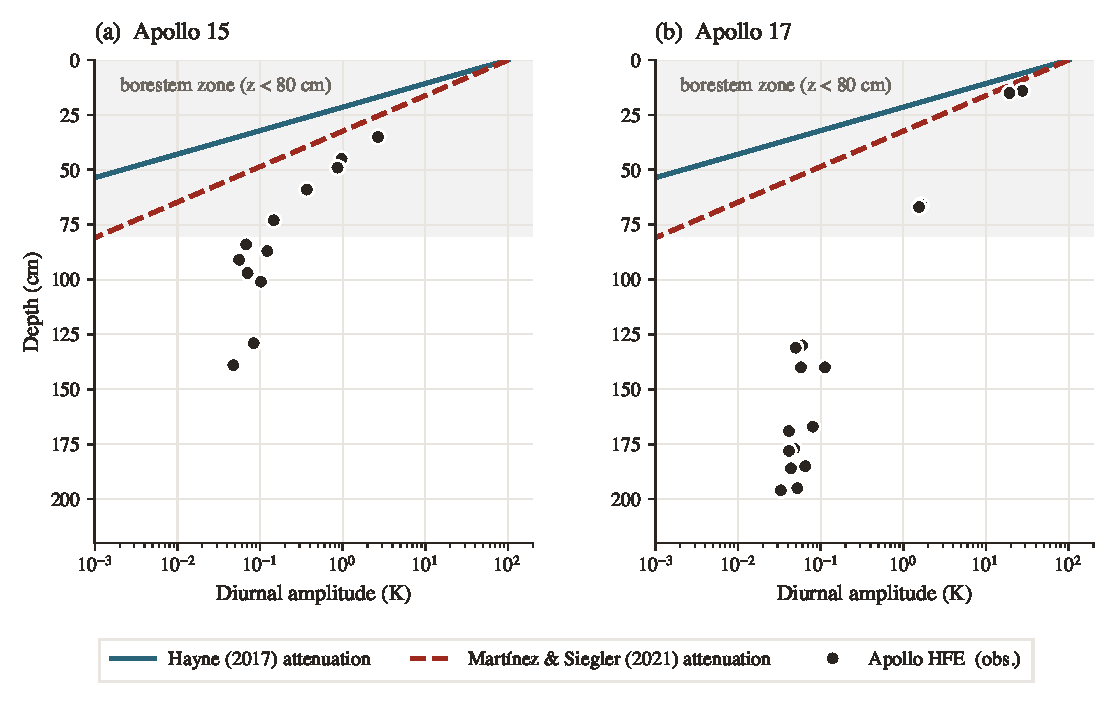
\includegraphics[width=\linewidth]{figures/apollo_amplitude_vs_depth.pdf}
\caption{Diurnal amplitude (half-range of the
local-solar-time-folded median temperature) versus sensor depth at
both Apollo sites. Black markers: observed; solid teal: \Hayne\
regolith attenuation; dashed red: \citet{martinez2021} attenuation,
both evaluated at $T=250$ K with the published deep-regolith density
of 1800 kg m$^{-3}$. The two model curves differ by $\sim$10\% in
predicted skin depth and are visually indistinguishable on the log
axis at all relevant depths. The shaded band is the borestem zone
($z<80$ cm). The order-of-magnitude shallow-sensor excess is the
borestem heat-short signature.}
\label{fig:amplitude}
\end{figure}

\subsection{Per-site $K_d$ retrieval (Hayne shape held
fixed)}\label{sec:methods-kd}
$K_d$ is retrieved separately at each site by minimising the
deep-sensor RMSE while holding the remainder of the Hayne
functional form (eqs.~\ref{eq:K}--\ref{eq:cp}) fixed.
$(K_s,H,\chi,T_\mathrm{ref})$ and the density and $c_p$ functions
are held at their published values, and $K_d$ is swept across
site-specific grids: 20 points spanning
1.5--$9.0\times10^{-3}\,\si{\watt\per\meter\per\kelvin}$ at A15
and 24 points spanning
3.0--$18.0\times10^{-3}\,\si{\watt\per\meter\per\kelvin}$ at A17.
The upper end of the A17 grid bounds the parabolic minimum; the
bootstrap upper tail (Fig.~\ref{fig:bootstrap}) extends slightly
beyond the swept range through parabolic extrapolation. At each
$K_d$ a full Crank--Nicolson spin-up is run to convergence, and
the deep-sensor RMSE is evaluated as
\begin{equation}
\mathrm{RMSE}(K_d) = \Bigl\langle\bigl[T_\mathrm{model}(z_i;K_d) - T_\mathrm{eq}^\mathrm{HFE}(z_i)\bigr]^2\Bigr\rangle_{z_i\ge\zborestem}^{1/2}.
\label{eq:rmse-kd}
\end{equation}
The point estimate $K_d^{*}$ is the parabolic minimum through the
three grid values bracketing $\arg\min\,\mathrm{RMSE}$. Its
uncertainty is quantified by a non-parametric bootstrap with
$N_\mathrm{boot}=1500$ resamples of the deep-sensor set drawn with
replacement, with the $\pm 2.5$ cm sensor-placement uncertainty
\citep{nagihara2018} propagated as a per-resample Gaussian depth
jitter, following standard small-sample regression practice
\citep{press2007}. The bootstrap distribution defines 95\%
confidence intervals on $K_d^{*}$ and on the inter-site contrast
$\Delta K_d^{*}$, and provides the null-hypothesis test for
inter-site equality (Fig.~\ref{fig:bootstrap}). Percentile-method
intervals are reported throughout; bias-corrected accelerated
(BCa) intervals \citep{efron1993} agree with the percentile
endpoints to within $1.3\,\si{\milli\watt\per\meter\per\kelvin}$
at both sites and on the contrast, and do not alter any
qualitative conclusion. The retrieval has one free parameter.

Models with different free-parameter counts on the same
deep-sensor set are compared using the small-sample-corrected
Akaike information criterion \citep{burnham2002},
$\mathrm{AICc}=N\ln(\mathrm{RSS}/N)+2k+2k(k{+}1)/(N{-}k{-}1)$,
where RSS is the deep-sensor residual sum of squares and $k$ is
the number of fitted parameters ($k=0$ for fixed-$K_d$ rows,
$k=1$ for each retrieval). Differences $\Delta\mathrm{AICc}$ are
reported relative to the best model at each site; following
\citet{burnham2002}, $\Delta\mathrm{AICc}\lesssim 2$ indicates
statistically indistinguishable models and
$\Delta\mathrm{AICc}\gtrsim 10$ a decisive preference. A reduced
$\chi^2$ is not reported: the within-stability-window scatter
($\sigma\sim 0.03$--$0.05$ K) characterises short-term
thermometer precision rather than the model-adequacy error
budget, yields $\chi^2_\nu\gg 1$ for every model, and is therefore
uninformative for model selection in this context.

% =====================================================================
\section{Results}\label{sec:results}

\subsection{Annual-mean subsurface profile and the global-model
gap}\label{sec:results-mean}
Neither published global model reproduces both Apollo boreholes
without per-site adjustment. Figure~\ref{fig:meanT} compares the
two modelled time-averaged $\langle T(z)\rangle$ profiles,
\citet{hayne2017} at the global
$K_d=3.4\,\si{\milli\watt\per\meter\per\kelvin}$ and
\citet{martinez2021} $K(T,\rho)$ evaluated forward, against the
stability-window means. The published Hayne value runs warm
relative to the HFE record by a mean of $+1.03$ K at A15 and
$+2.88$ K at A17; the \citet{martinez2021} prediction is closer at
both sites but underpredicts A17 by $\sim$2 K
(Table~\ref{tab:headline}). The shaded band ($z<\zborestem$) marks
the borestem-contaminated zone, excluded \emph{a priori} from the
quantitative comparison (\S\ref{sec:borestem}). The residual
that remains motivates the per-site $K_d$ retrieval of
\S\ref{sec:results-kd}.

\begin{figure}[!htbp]
\centering
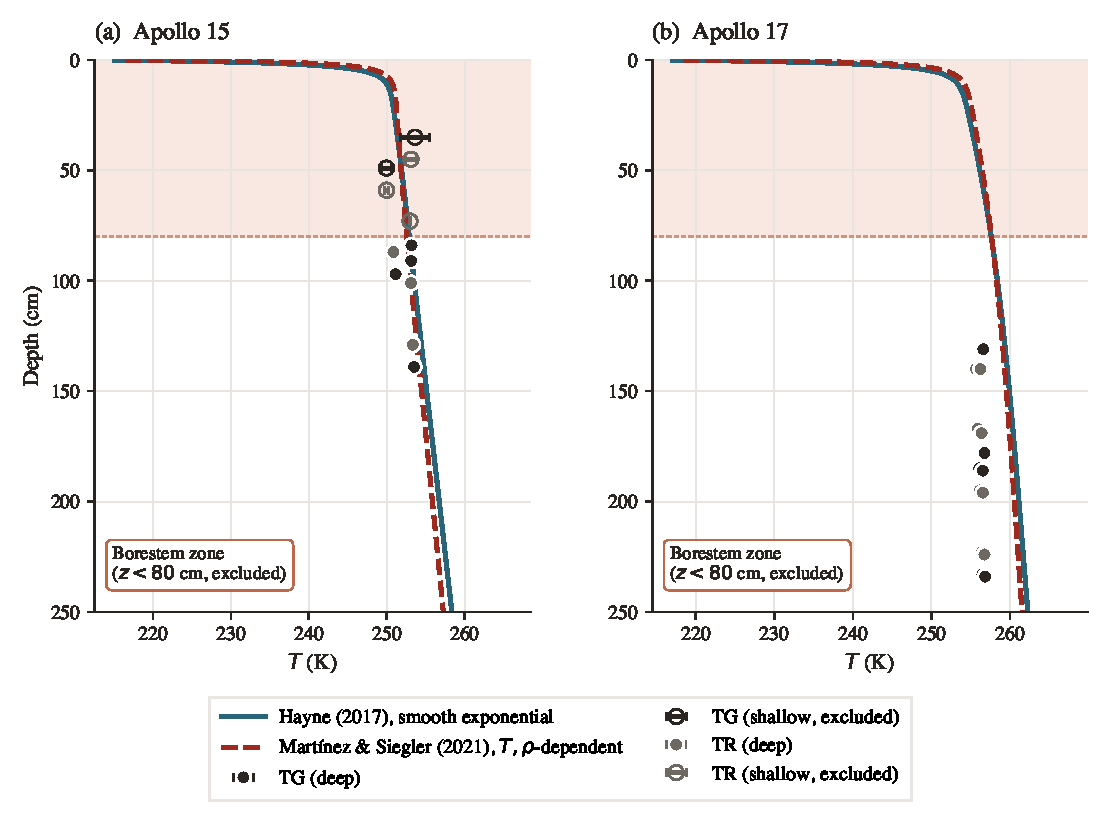
\includegraphics[width=\linewidth]{figures/fig2_apollo_mean_T_profile.pdf}
\caption{Annual-mean subsurface temperature $\langle T(z)\rangle$ for
the two published conductivity models at their nominal (un-retrieved)
parameters, \Hayne\ smooth exponential at the global
$K_d=3.4\,\si{\milli\watt\per\meter\per\kelvin}$ (solid), and the
\citet{martinez2021} temperature- and density-dependent $K(T,\rho)$
forward (dashed), against the Apollo HFE stability-window means.
Markers are coded by sensor type (charcoal $=$ TG, grey $=$ TR);
horizontal bars are the within-window standard deviation. The shaded
band is the borestem-contaminated zone ($z<\SI{80}{\centi\meter}$),
excluded from the RMSE.}
\label{fig:meanT}
\end{figure}

\begin{table}[t]
\centering
\small
\setlength{\tabcolsep}{5pt}
\caption{\textbf{Headline deep-sensor RMSE table.} Deep-sensor
($z>80$ cm) validation statistics for the three forward
configurations confronted with the same Apollo HFE record: the
\Hayne\ form at its published global $K_d$, the \Hayne\ form
with $K_d$ refit per site (the retrieval of
\S\ref{sec:results-kd}), and the \citet{martinez2021}
$K(T,\rho)$ model evaluated forward at each site. $K_d$ in
mW m$^{-1}$ K$^{-1}$ (95\% bootstrap CI in brackets for the
Hayne site-fit row). Bias $=$ mean(model $-$ obs). A
diagnostic per-site retrieval under the \citet{martinez2021}
form is presented separately in \S\ref{sec:disc-prior}.}
\label{tab:headline}
\begin{tabular}{l l l c c c}
\toprule
Site & Model & Fitted knob & $N$ & RMSE (K) & Bias (K) \\
\midrule
Apollo 15 & Hayne (2017), global $K_d$    & ---                              & 7  & \textbf{1.37} & $+1.03$ \\
Apollo 15 & Hayne, $K_d^{*}$ fit          & $K_d^{*}=4.86\,[3.94,14.36]$     & 7  & \textbf{0.91} & $+0.00$ \\
Apollo 15 & \citet{martinez2021} forward  & ---                              & 7  & \textbf{1.10} & $+0.60$ \\
\midrule
Apollo 17 & Hayne (2017), global $K_d$    & ---                              & 16 & \textbf{2.96} & $+2.88$ \\
Apollo 17 & Hayne, $K_d^{*}$ fit          & $K_d^{*}=11.23\,[10.18,21.62]$   & 16 & \textbf{0.30} & $-0.03$ \\
Apollo 17 & \citet{martinez2021} forward  & ---                              & 16 & \textbf{2.47} & $+2.30$ \\
\bottomrule
\end{tabular}
\end{table}

\label{sec:headline-table}

\subsection{Per-site $K_d$ retrieval}\label{sec:results-kd}
The deep-sensor RMSE exhibits a well-resolved minimum at each site:
\[
K_{d,\mathrm{A15}}^{*}=4.86^{+1.12}_{-0.54}\,[3.94,\,14.36]\,\si{\milli\watt\per\meter\per\kelvin},\qquad
K_{d,\mathrm{A17}}^{*}=11.23^{+8.12}_{-0.77}\,[10.18,\,21.62]\,\si{\milli\watt\per\meter\per\kelvin},
\]
with asymmetric $1\sigma$ bootstrap uncertainties and 95\%
confidence intervals in brackets (Fig.~\ref{fig:bootstrap}). The
deep-sensor RMSE decreases from 1.37 K and 2.96 K under the
published global $K_d$ to 0.91 K and 0.30 K under the per-site
retrieval ($N=7$ at A15, $N=16$ at A17;
Table~\ref{tab:headline}), and the residual bias falls to
$\le 0.03$ K. $K_d$ is therefore the dominant identifiable lever
between the Hayne form and the in-situ HFE record once the
borestem zone is excluded.

The minimum is not an artefact of the sweep grid. Extending the
sweep beyond the fitting envelope reveals that each RMSE curve
rises monotonically on the high-$K_d$ side
(Fig.~\ref{fig:kdsweep}), confirming bracketed minima rather than
descending shoulders. A fivefold refinement of the grid around
each minimum, combined with a factor-of-two tightening of the
spin-up length and convergence tolerance (60 lunations to
$5\times10^{-3}$ K versus the production 30 lunations to
$5\times10^{-2}$ K), shifts $K_d^{*}$ by less than
$0.10\,\si{\milli\watt\per\meter\per\kelvin}$ at both sites,
well within the bootstrap uncertainty quoted above.

The \citet{martinez2021} model, evaluated forward at each site
with its published global coefficients, serves as the
global-baseline comparison: deep-sensor RMSE of 1.10 K at A15
and 2.47 K at A17, with mean biases of $+0.6$ K and $+2.3$ K
(Table~\ref{tab:headline}). It reproduces A15 to within a factor
of $\sim$1.2 of the Hayne site-fit RMSE but underpredicts A17 by
an amount comparable to the Hayne global miss, as expected
for a globally calibrated $K(T,\rho)$ without per-site freedom.
A diagnostic per-site retrieval under this form is presented in
\S\ref{sec:disc-prior}, where the implications for the
$K(T,\rho)$ parameterization are discussed.

\paragraph*{Sensitivity to the borestem exclusion depth.}
The retrieval is repeated with the borestem exclusion depth
$z_b$ swept over 60--90 cm. The retrieved values remain stable
across all admissible cuts:
$K_{d,\mathrm{A15}}^{*}=4.7$--$4.9$ and
$K_{d,\mathrm{A17}}^{*}=11.2\,\si{\milli\watt\per\meter\per\kelvin}$
for $z_b=70$, 80, and 90 cm, yielding a contrast of
6.3--$6.5\,\si{\milli\watt\per\meter\per\kelvin}$, unchanged
within rounding from the nominal value. The 60 cm cut alone
deviates ($K_{d,\mathrm{A17}}^{*}=18.8$, contrast 14.2),
because at this depth a sensor inside the borestem-affected zone
re-enters the A17 set and inflates the retrieved gradient,
precisely the contamination that the amplitude-based cut
(\S\ref{sec:borestem}) is designed to exclude. The retrieval is
therefore insensitive to $z_b$ across its physically defensible
range, and the 60 cm outlier confirms rather than undermines the
borestem diagnostic.

\begin{figure}[!htbp]
\centering
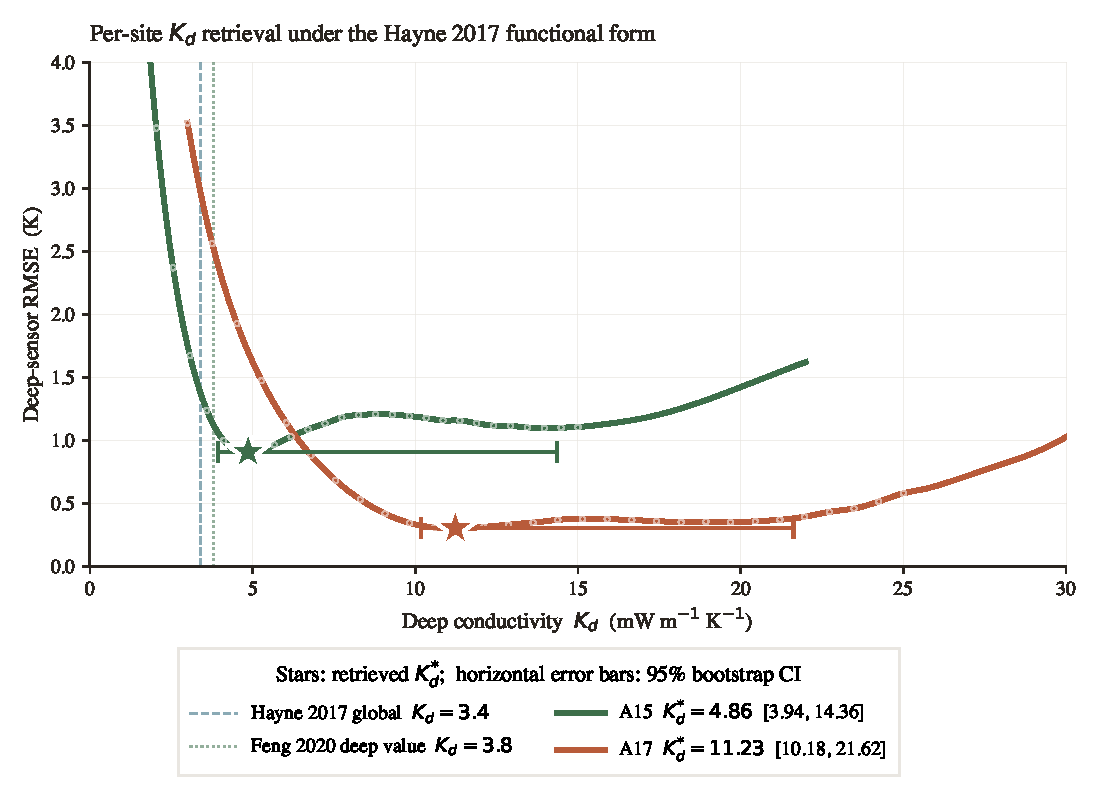
\includegraphics[width=\linewidth]{figures/fig5_kd_sweep.pdf}
\caption{Per-site $K_d$ retrieval under the \Hayne\ functional form,
with all other \Hayne\ parameters held at their published values.
Deep-sensor RMSE($K_d$) at each site, extended past the fitting grid
so each curve is shown rising again on the high-$K_d$ side: the
minima are genuine bracketed bowls, not descending shoulders.
Markers: forward-model evaluations; stars: retrieved $K_d^{*}$;
shaded band: 95\% bootstrap CI. Dashed vertical: \citet{hayne2017}
global $K_d=3.4$; dotted: the \citet{feng2020} deep value $K_d=3.8$.}
\label{fig:kdsweep}
\end{figure}

Two summary statistics must be distinguished. The $K_d^{*}$ values
quoted above are parabolic point estimates of the RMSE minimum;
the bootstrap medians of the same quantities are 4.88 and
$11.51\,\si{\milli\watt\per\meter\per\kelvin}$
(Table~\ref{tab:errorbudget}), marginally higher because each
bootstrap distribution is right-skewed. The inter-site contrast is
defined as the bootstrap median of the paired within-resample
difference,
$\Delta K_d^{*} = 6.63^{+7.43}_{-1.25}\,\si{\milli\watt\per\meter\per\kelvin}$
($1\sigma$, asymmetric; 95\% CI $[-3.2,\,16.6]$,
$p\approx 0.05$ for the null of inter-site equality;
Fig.~\ref{fig:bootstrap}). The paired construction preserves the
resample-level correlation between sites and is therefore the
statistically appropriate estimator; this is also the reason 6.63
differs slightly from the difference of the point estimates
($11.23-4.86=6.37$). The broad A15 upper tail reflects a weakly
constrained shoulder in RMSE$(K_d)$ at A15 for $N=7$ deep
sensors, even though the central parabolic minimum is firmly at
4.86. The reported $1\sigma$ intervals propagate sensor-set
composition, the $\pm 2.5$ cm depth-placement uncertainty
\citep{nagihara2018}, and the parabolic curve-fit error;
component-by-component impacts of the remaining Hayne inputs are
tabulated in Table~\ref{tab:errorbudget}. Both retrievals reject
the global $K_d=3.4\,\si{\milli\watt\per\meter\per\kelvin}$ of
\citet{hayne2017} at the 95\% level.

\begin{figure}[!htbp]
\centering

\includegraphics[width=\linewidth]{figures/fig_bootstrap.pdf}
\caption{\textbf{Bootstrap distributions
($N_\mathrm{boot}=1500$, deep-sensor resampling with $\pm 2.5$\,cm
depth jitter).} (a)~Per-site $K_d^{*}$ histograms with 95\% CIs in the
legend; dashed vertical at the \citet{hayne2017} global value. (b)~
Inter-site contrast $\Delta K_d^{*}\!=\!K_d^{\rm A17}\!-\!K_d^{\rm A15}$;
95\% CI shaded, lower bound just touching zero
($p\!\approx\!0.05$).}
\label{fig:bootstrap}
\end{figure}

Applied at each site, the retrieved $K_d^{*}$ values yield
deep-sensor profiles that track the HFE observations within the
$\sim 1$ K spread of the data
(Fig.~\ref{fig:thermal-profiles}). The \citet{martinez2021}
forward, plotted alongside, reproduces A15 to within a factor of
$\sim$1.2 of the Hayne site-fit but underpredicts A17.

\begin{figure}[!htbp]
\centering
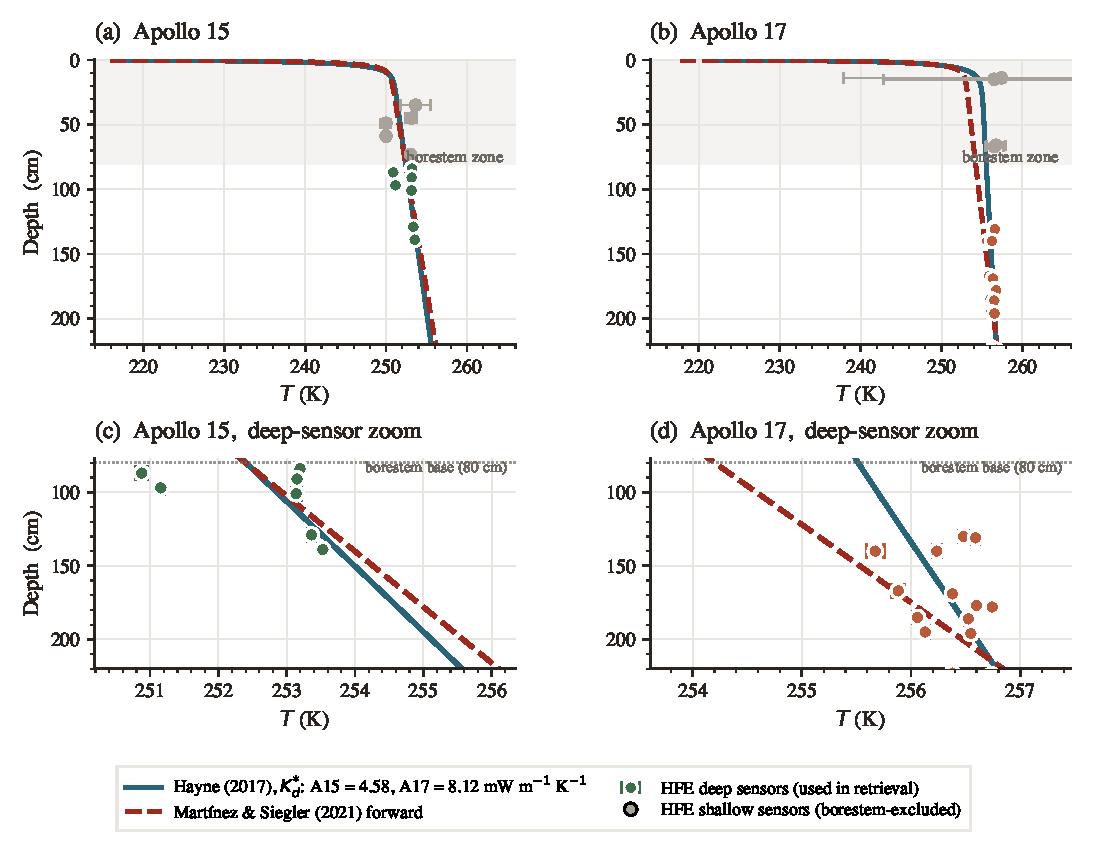
\includegraphics[width=\linewidth]{figures/fig_thermal_profiles.pdf}
\caption{Annual-mean $T(z)$ at the two sites under the two
conductivity models, against the Apollo HFE deep sensors. Solid
teal: \Hayne\ at the per-site retrieved $K_d^{*}$; dashed red:
\citet{martinez2021} forward (no fitted knob). Top: full profile;
bottom: deep-sensor zoom. Coloured markers: HFE deep sensors
(used in retrieval); grey markers: borestem-affected shallow
sensors (excluded).}
\label{fig:thermal-profiles}
\end{figure}

A full per-component error budget for $K_d^{*}$ is deferred to
\S\ref{sec:disc-degeneracy} (Table~\ref{tab:errorbudget}),
where the basal-flux degeneracy that dominates the budget is
discussed.

\subsection{Consistency checks}\label{sec:consistency}
Three diagnostics test the per-site $K_d^{*}$ values. Their
status as independent or internal is identified explicitly.

An independent Diviner surface-temperature closure test
(Fig.~\ref{fig:diviner}, discussed in \S\ref{sec:disc-prior})
shows that both conductivity models reproduce the canonical
lunar diurnal shape, confirming that the diurnal forcing chain
is correctly captured. Two further internal checks follow.

\emph{(i) TG vs.\ TR cross-prediction.} Fitting $K_d$ on the
gradient-bridge sensors (TG) alone and predicting the
ring-bridge (TR) sensors, and vice versa, yields held-out RMSEs
within $\sim$0.25 K of the in-sample values at both sites.
\emph{(ii) Leave-one-deepest-out.} Withholding the deepest
sensor ($z=139$ cm at A15, $z=234$ cm at A17) and refitting
$K_d$ on the remainder predicts the held-out temperature to
within $|\Delta|=0.31$ K and $|\Delta|=0.16$ K respectively.
Both internal checks confirm that the retrieval is not driven by
a single sensor or sensor type; neither constitutes an
independent test of the inter-site contrast.

\emph{Bayesian cross-check.} The non-parametric
bootstrap is reported as the primary uncertainty estimate
throughout because it makes no assumption about the basal heat
flux and propagates only quantities measured at the boreholes
(sensor-set composition and placement depth). As an independent
cross-check on the \emph{direction} of the contrast, not as a
second estimate of its magnitude, we also ran a Bayesian
inversion propagating the \citet{saito2007,nagihara2018} prior
on $Q_b$. Its marginal MCMC medians are
$K_{d,\mathrm{A15}}=3.9$ and $K_{d,\mathrm{A17}}=13.1$
mW m$^{-1}$ K$^{-1}$ (contrast median $+9.2$). These differ
from the bootstrap point estimates (4.86, 11.23; contrast
$+6.6$) by construction, not by disagreement: the $Q_b$ prior
slides each marginal along the $K_d/Q_b$ degeneracy ridge
(\S\ref{sec:disc-kd}), so the two methods are not independent
measurements of the absolute $K_d$. They agree on the ordering,
$P(K_d^{\rm A17}>K_d^{\rm A15})\approx 96\%$, since the
degeneracy ridge shifts both sites together. The bootstrap
interval on the contrast magnitude ($\Delta K_d^{*}=6.6$,
95\% CI $[-3.2,16.6]$) is carried forward as the headline
measurement.

% =====================================================================
\FloatBarrier
\section{Discussion}\label{sec:discussion}

\subsection{The two boreholes require different deep
gradients}\label{sec:disc-kd}
The HFE record does not admit a single deep conductivity that
fits both sites. Under the Hayne form at the published basal
heat fluxes, the value that zeroes the A17 deep-sensor residual
(11.23) overcorrects A15 to $-0.50$ K, and the value that zeroes
A15 (4.86) leaves A17 warm by $+1.63$ K. The published global
value of \citet{hayne2017}, applied unchanged, runs warm at both
sites but by significantly different amounts ($+1.03$ K at A15,
$+2.88$ K at A17; Table~\ref{tab:headline}). The per-site
retrievals are
$K_d^{\mathrm{A15}}=4.86$ and
$K_d^{\mathrm{A17}}=11.23\,\si{\milli\watt\per\meter\per\kelvin}$
(95\% bootstrap CIs $[3.94,\,14.36]$ and $[10.18,\,21.62]$). The
lower 95\% bound on the contrast distribution
(Fig.~\ref{fig:bootstrap}b) coincides with zero
($p\approx 0.05$); the \emph{magnitude} of the contrast is
therefore not established at the 95\% level by two boreholes
alone, but the \emph{requirement} of different deep gradients is.

The pooled three-model comparison (Table~\ref{tab:modelcomp})
confirms this conclusion directly. A per-site $K_d$ with $Q_b$
fixed at the published values (M1) is preferred over a shared
$K_d$ with per-site $Q_b$ free within the published envelope (M2)
and over the strict null of shared $K_d$ and fixed $Q_b$ (M3) by
$\Delta\mathrm{AICc}\approx 5$. Under the standard interpretation
of the small-sample AIC, this constitutes ``considerably less
support'' for the alternatives but is not decisive; M2 attains
its best fit only by driving the two basal fluxes to opposite
extremes of their published ranges, the least probable
configuration within the envelope. The data therefore favor a
per-site difference in deep gradient without excluding a
uniform-conductivity alternative in which the two basal heat
fluxes differ.

\begin{table}[!htbp]
\centering
\small
\caption{Pooled deep-sensor model comparison ($N=23$: $7$ at A15,
$16$ at A17). M1 retrieves a per-site $K_d$; M2 shares one $K_d$ and
frees the per-site $Q_b$ within the published envelope; M3 fixes
both. $\Delta$AICc is relative to the best model. $K_d$ in
mW\,m$^{-1}$\,K$^{-1}$, $Q_b$ in mW\,m$^{-2}$.}
\label{tab:modelcomp}
\begin{tabular}{llccc}
\toprule
Model & $K_d$ (A15\,/\,A17) & $Q_b$ (A15\,/\,A17) & RMSE (K) & $\Delta$AICc \\
\midrule
M1\ \ variable $K_d$, $Q_b$ fixed & $5.0$\,/\,$11.0$ & $21$\,/\,$15$ (fixed) & \textbf{0.56} & \textbf{0.0} \\
M2\ \ uniform $K_d$, $Q_b$ free   & $6.5$ (shared)   & $25$\,/\,$10$ (fitted) & 0.59 & $+5.1$ \\
M3\ \ uniform $K_d$, $Q_b$ fixed  & $13.0$ (shared)  & $21$\,/\,$15$ (fixed) & 0.67 & $+5.7$ \\
\bottomrule
\end{tabular}
\end{table}

\subsection{The retrieved absolute $K_d$ values are
degeneracy-limited}\label{sec:disc-degeneracy}
The absolute $K_d^{*}$ values must be interpreted as conditional
on the adopted basal heat flux, not as free-standing
measurements. At steady state, the deep gradient
$|\partial_z T|=Q_b/K_d$ is invariant under any rescaling
$(K_d,Q_b)\!\to\!(\alpha K_d,\alpha Q_b)$: a single borehole
cannot resolve these two products independently. The degeneracy
is mapped quantitatively in Fig.~\ref{fig:robustness}a and is
visible in the joint Bayesian posteriors. Adopting the canonical
$Q_b^{\mathrm{A17}}=15\,\si{\milli\watt\per\meter\squared}$
\citep{langseth1976,nagihara2018} yields $K_d=11.23$;
substituting the lower
$\sim$10 mW m$^{-2}$ value of \citet{saito2007,nagihara2018}
rescales $K_d$ downward to $\sim$7.7
mW m$^{-1}$ K$^{-1}$, while the upper bound $\sim$18 mW m$^{-2}$
shifts it upward to $\sim$13.8
mW m$^{-1}$ K$^{-1}$. The A17 $K_d^{*}$ therefore carries a
$\sim\pm 40\%$ envelope determined entirely by the basal-flux
debate; A15 carries a comparable envelope. The quantity
constrained tightly at each borehole is the product $Q_b/K_d$,
equivalently the deep gradient itself. This represents the
intrinsic limit of what two boreholes can deliver.

\begin{table}[!htbp]
\centering
\footnotesize
\setlength{\tabcolsep}{4pt}
\renewcommand{\arraystretch}{1.10}
\caption{\textbf{Per-component $1\sigma$ error budget for
$K_d^{*}$.} Values in mW m$^{-1}$ K$^{-1}$; entries below 0.05
are reported as $<\!0.05$. The total is the
independent-errors quadrature sum
$\sigma_{\rm tot}=\sqrt{\sum_i \sigma_i^2}$.}
\label{tab:errorbudget}
\begin{tabular}{@{}l p{0.20\linewidth} p{0.30\linewidth} r r@{}}
\toprule
Component & Envelope & Method & A15 & A17 \\
\midrule
\multicolumn{5}{@{}l}{\textit{Data-side (bootstrap + measured inputs)}} \\[2pt]
$\sigma_\mathrm{stat}$
  & $\pm 2.5$\,cm depth jitter
  & bootstrap 16--84 \% half-range
  & 0.83 & 4.44 \\
$\sigma_A$\,(albedo)
  & $A\!\pm\!0.01$
  & re-retrieve $K_d^{*}$ at perturbed $A$
  & 0.07 & 0.54 \\
\midrule
\multicolumn{5}{@{}l}{\textit{Input-parameter uncertainty (Hayne coefficients)}} \\[2pt]
$\sigma_{Q_b}$
  & $Q_b$\,A15$\in\![14,25]$,\,A17$\in\![10,18]$
  & $K_d/Q_b$ degeneracy mapping
  & 1.47 & 3.45 \\
$\sigma_\chi$
  & $\chi\!\in\![1.48,2.7]$
  & re-retrieve at each endpoint
  & 0.69 & 2.03 \\
$\sigma_H$
  & $H\!\in\![1,11]$\,cm
  & half-range of per-$H$ $K_d^{*}$ on $11\!\times\!8$ grid
  & 0.31 & 1.44 \\
$\sigma_{K_s}$
  & $K_s\!\pm\!30\%$
  & re-retrieve at perturbed $K_s$
  & 0.06 & $<\!0.05$ \\
\midrule
\multicolumn{5}{@{}l}{\textit{Methodological choices (this work)}} \\[2pt]
$\sigma_\mathrm{thr}$
  & $0.04$--$0.16$\,K/yr ($4\!\times$ adopted)
  & threshold sweep, max $|\Delta K_d^{*}|$
  & 0.03 & 0.11 \\
$\sigma_{z_b}$
  & $z_b\!\in\!\{70,80,90\}$\,cm
  & cut sweep, half-range of $K_d^{*}$
  & 0.10 & $<\!0.05$ \\
\midrule
\multicolumn{5}{@{}l}{\textit{Excluded by structure}} \\[2pt]
$\sigma_\rho$
  & $\rho_d\!\in\![1700,2000]$\,kg\,m$^{-3}$
  & no explicit $\rho$ in Hayne $K(T,z)$ (eq.~\ref{eq:K})
  & 0.00 & 0.00 \\
\midrule
\textbf{Total (quadrature)} & & & \textbf{1.86} & \textbf{6.17} \\
Bootstrap median $K_d^{*}$  & & & 4.88 & 11.51 \\
\bottomrule
\end{tabular}
\end{table}

\paragraph*{Reading the per-component error budget.}
The derivation of each row in Table~\ref{tab:errorbudget} falls
into one of three categories: $\sigma_\mathrm{stat}$ is the
16--84 percentile half-width of the bootstrap distribution
under the $\pm 2.5$ cm astronaut-emplacement envelope reported
by \citet{nagihara2018};
$\sigma_{Q_b}$ is obtained in closed form through the $K_d/Q_b$
degeneracy across the published reduction range
(\citealp{langseth1976} canonical;
\citealp{saito2007,nagihara2018} reanalysis); every remaining
row is computed by re-running the full retrieval at the
perturbed input. The non-bootstrap envelopes themselves are
taken from the published literature: $\sigma_A$ uses the
\citet{vasavada2012} lat-band scatter on the Bond albedo;
$\sigma_\chi$ uses the actual Vasavada--Hayne disagreement
(\citealp{hayne2017} Appendix~A adopts $\chi=2.7$;
\citealp{vasavada2012} use $\chi^{*}=1.48$ under their
normalisation, a factor of $\sim$1.8 that exceeds any $\pm 30\%$
approximation); $\sigma_{K_s}$ uses the \citet{cremers1971}
laboratory scatter on Apollo~11 fines as a generous upper bound,
since \citet{hayne2017} adopt
$K_s=\SI{7.4e-4}{\watt\per\meter\per\kelvin}$ without a published
uncertainty and these are the only laboratory data known to us
for lunar regolith; the $\sigma_\rho$ envelope is the
\citet{mitchell1973,carrier1991} Apollo-core compaction range.

\emph{How the total is combined.} The \textbf{Total (quadrature)}
row is the independent-errors combination
$\sigma_{\rm tot}=\sqrt{\sum_i \sigma_i^2}$, not the linear sum
$\sum_i \sigma_i$. For A15 the worked arithmetic is
\begin{equation*}
\begin{aligned}
\sigma_{\rm tot}^{\rm A15} &=
\big(0.83^{2}+0.07^{2}+1.47^{2}+0.69^{2}+0.31^{2}\\
&\quad{}+0.06^{2}+0.03^{2}+0.10^{2}+0^{2}\big)^{1/2}\\
&= \sqrt{3.44}\;=\;1.86~\text{mW m}^{-1}\,\text{K}^{-1};
\end{aligned}
\end{equation*}
the corresponding linear sum $\sum_i \sigma_i = 3.30$ would be
the appropriate combination only under perfectly correlated
worst-case errors, which we do not assume. The 1.86 (A15) and
6.17 (A17) totals therefore represent the standard quadrature
combination of nominally independent components, and the same
arithmetic at A17 gives
\begin{equation*}
\sigma_{\rm tot}^{\rm A17} =
\big(4.44^{2}+0.54^{2}+3.45^{2}+2.03^{2}+1.44^{2}+0.05^{2}+0.11^{2}+0.05^{2}\big)^{1/2}
\approx 6.17.
\end{equation*}
We flag one residual correlation: $\sigma_\mathrm{stat}$ and
$\sigma_{Q_b}$ are not strictly independent because both
propagate along the $K_d/Q_b$ degeneracy ridge of
Fig.~\ref{fig:robustness}a, so 1.86 and 6.17 should be read as
the independence-idealised totals rather than as fully
decorrelated standard errors; the practical effect on the
absolute $K_d^{*}$ envelope is small because the $Q_b$ envelope
dominates the budget at both sites in any case.

Three conclusions follow. First, $\sigma_{Q_b}$ and
$\sigma_\mathrm{stat}$ together account for $\sim$91\% of the
quadrature sum at both sites, with the remaining $\sim$9\%
split between $\sigma_\chi$ and (at A17) $\sigma_A$. Second,
$\sigma_\rho$ is identically zero under the Hayne $K(T,z)$ form
(eq.~\ref{eq:K}), which contains no explicit $\rho$ dependence:
$\rho(z)$ enters only the volumetric heat capacity $\rho c_p$,
which controls the transient response and not the steady-state
deep gradient. A wider Apollo-core $\rho$ envelope therefore
does not broaden $K_d^{*}$ under this $K$-form; the row is
retained to record this structural property. Third, the
methodological-choice rows $\sigma_\mathrm{thr}$ and
$\sigma_{z_b}$ sit an order of magnitude below the data-side
and parameter terms, indicating robustness against both
discretionary cuts.

\paragraph*{Behaviour of the inter-site contrast under independent
$Q_b$ revision.}
The inter-site contrast is far less sensitive to $Q_b$ than the
absolute $K_d^{*}$ values, because a uniform rescaling
$(K_d,Q_b)\!\to\!(\alpha K_d,\alpha Q_b)$ cancels exactly in
$\Delta K_d^{*}$; the contrast is exposed to $Q_b$ uncertainty
only through the differential between the two sites' rescaling
factors. We test this explicitly by rescaling $Q_b$
independently at the two sites across the full published
envelope ($Q_{b,\mathrm{A15}}\in[14,25]$,
$Q_{b,\mathrm{A17}}\in[10,18]$ mW m$^{-2}$;
Fig.~\ref{fig:robustness}a). Along the global-rescaling
diagonal, the contrast is invariant at its nominal value of
6.6 mW m$^{-1}$ K$^{-1}$. Off the diagonal, the most adverse
combination, A15 at the upper end of its $Q_b$ envelope and
A17 at the lower end, compresses the contrast to
$\Delta K_d^{*}\approx 1.9$ mW m$^{-1}$ K$^{-1}$
($\sim$0.4 $\sigma$); the opposite extreme expands it to
$\sim$10.6. The sign of the contrast is preserved throughout
the published $Q_b$ envelope: A17 remains the more conductive
site under every admissible per-site basal-flux assignment. The
contrast magnitude is therefore not statistically significant
under arbitrary independent $Q_b$ revisions, a $-33\%$
revision of $Q_{b,\mathrm{A17}}$ alone, for instance, suffices
to reduce it below $1\sigma$, but its sign is robust, and
that sign underpins the central conclusion that no single
globally uniform $K_d$ reproduces both records.

A joint $(K_d, H)$ fit over the swept $H = 1$--11 cm range
(Fig.~\ref{fig:robustness}b,c) confirms that $H$ is
effectively unconstrained: the RMSE surface varies by
$<\!0.02$ K across $H=3$--11 cm, with shallow interior minima
at $H\approx 10$ cm (A15) and 4 cm (A17). The retrieved $K_d$
is nonetheless stable, the joint minimum and the 1-parameter
retrieval at $H=6$ cm agree in $K_d$ to within the 0.5 K RMSE
contour. $K_d$, not $H$, is the identified parameter.

\begin{figure}[!htbp]
\centering

\includegraphics[width=\linewidth]{figures/fig_robustness.pdf}
\caption{Robustness of the per-site $K_d^{*}$ contrast.
\textbf{(a)} Contrast $\Delta K_d^{*}$ as a function of
per-site $Q_b$ rescaling factors $\alpha_{15},\alpha_{17}$.
Solid diagonal: global rescaling; dashed contours:
bootstrap-$\sigma$ significance; black circle: nominal $Q_b$;
green square: \citet{saito2007} A15 reanalysis.
\textbf{(b),(c)} Joint $(K_d, H)$ RMSE surface at each site.
Coral diamond: joint RMSE minimum; teal circle: 1-parameter
retrieval at $H=6$ cm.}
\label{fig:robustness}
\end{figure}

\subsection{Comparison with Mart{\'\i}nez \& Siegler (2021) and
prior estimates}\label{sec:disc-prior}
A second globally calibrated $K(T,\rho)$ form fails in the same
direction as the first when evaluated forward. The
\citet{martinez2021} model, with its published coefficients,
yields a deep-sensor RMSE of 1.10 K at A15 and 2.47 K at A17
(Table~\ref{tab:headline}, Fig.~\ref{fig:thermal-profiles}): A15
within a factor of $\sim$1.2 of the Hayne site-fit, A17
underpredicted by an amount comparable to the Hayne global miss.
Both models inherit the same globally averaged thermal structure
(both are calibrated against the same family of orbital Diviner
products), and the implication for any single global $K(T,z)$ is
identical: per-site freedom is required to reproduce both Apollo
boreholes simultaneously.

\paragraph*{Diagnostic: Martinez per-site density retrieval.}
The fairness of the forward Martinez comparison can be tested by
granting the published $K(T,\rho)$ one per-site lever and asking
whether that lever can absorb the A17 residual within physical
bounds. We note at the outset that \citet{martinez2021}
calibrated their four coefficients against surface
brightness-temperature observations and did not validate the
extrapolation to depths of order one meter; the test we run
here is therefore a check of whether the published surface-
calibrated form, when extended to the deep regolith, can fit
the in-situ HFE data with one per-site lever (the deep bulk
density entering the model). We do so under the construction
of \S\ref{sec:methods-kd} (eq.~\ref{eq:alpha}): rescale the
deep asymptote of the Hayne-form $\rho(z)$ entering
equation~(\ref{eq:K-ms}) by a single per-site scalar $\alpha$,
leaving the four Martinez coefficients fixed, and sweep
$\alpha$ against the same deep-sensor RMSE. The retrieved values are
$\alpha^{*}_{\mathrm{A15}}=1.12$ (deep bulk density
$\rho_d^{*}\approx 2010$ kg m$^{-3}$, RMSE 0.91 K) and
$\alpha^{*}_{\mathrm{A17}}=1.83$ ($\rho_d^{*}\approx 3300$
kg m$^{-3}$, RMSE 0.31 K), both matching the Hayne site-fit RMSE
to within $\sim$0.01 K. The physical interpretation of $\alpha$
is the deep bulk density that the published Martinez $K(T,\rho)$
would require to reproduce each site's in-situ profile.

The A15 retrieval sits marginally above the Apollo-core
compaction ceiling of $\sim$2000 kg m$^{-3}$
\citep{mitchell1973,carrier1991} but remains physically
plausible. The A17 retrieval lies well above any admissible
regolith density: solid lunar basalt is $\sim$3000 kg m$^{-3}$
\citep{wieczorek2006}, and the 0.30--0.45 porosities measured in
Apollo cores cap the deep regolith asymptote near $\sim$2100
kg m$^{-3}$. The published Martinez form therefore cannot
reproduce the A17 deep profile under any physically defensible
density at the canonical $Q_b$. Within the $K_d/Q_b$ degeneracy
of \S\ref{sec:disc-degeneracy} this does not isolate
conductivity from basal flux at A17, the same A17 deep
gradient at a lower $Q_b$ would require less extreme densities
but at the canonical $Q_b$ the published Martinez
density-dependence is structurally insufficient on its own to
absorb the A17 deep gradient.
Figure~\ref{fig:alpha-sweep} visualises the result: the A15
RMSE($\alpha$) bowl bottoms inside the Apollo-core admissible
band, while the A17 bowl bottoms well outside it, between the
Apollo-core ceiling and the solid-basalt upper bound.

\begin{figure}[!htbp]
\centering
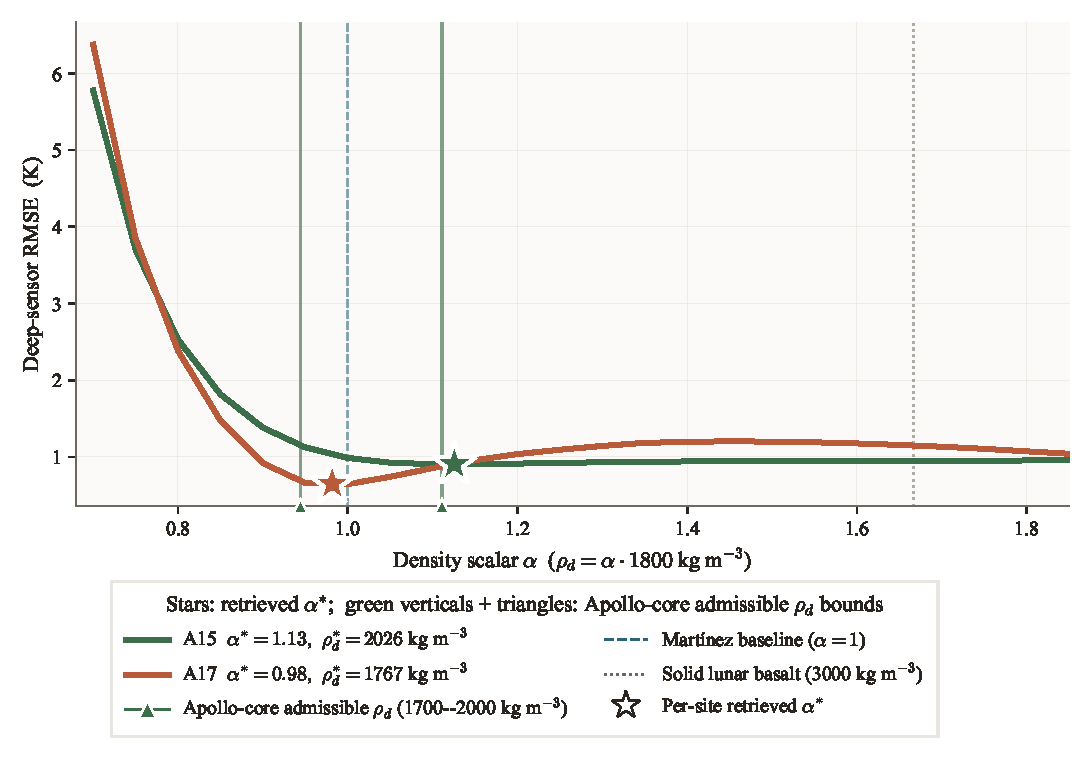
\includegraphics[width=\linewidth]{figures/fig_alpha_sweep.pdf}
\caption{Diagnostic per-site retrieval under the
\citet{martinez2021} $K(T,\rho)$ form. Deep-sensor RMSE as a
function of the per-site density scalar $\alpha$
(eq.~\ref{eq:alpha}) at \textbf{(a)} Apollo 15 and
\textbf{(b)} Apollo 17. Dashed teal: published Martinez
baseline ($\alpha=1$, $\rho_d=1800$ kg m$^{-3}$). Green band:
Apollo-core admissible density range
($\rho_d=1700$--$2000$ kg m$^{-3}$;
\citealp{mitchell1973,carrier1991}). Dotted grey:
solid-basalt upper bound (3000 kg m$^{-3}$;
\citealp{wieczorek2006}).}
\label{fig:alpha-sweep}
\end{figure}

The inferred ratio
$K_d^{\mathrm{A17}}/K_d^{\mathrm{A15}}\approx 2$ is large but
physically plausible if interpreted as a conductivity effect. Two
mechanisms act in the appropriate direction. First, Apollo cores
span bulk porosities $\phi\sim 0.30$--0.45
\citep{mitchell1973,carrier1991}; the effective-medium scaling
$K_\mathrm{eff}\propto(1-\phi)^2$ of \citet{wood2020} accounts
for a factor of $\sim$1.5 change at the upper end of that
range. Second, solid lunar basalt is $\sim$30\% more conductive
than solid highland anorthosite \citep{horai1972}, and A17 lies
in a basaltic embayment while A15 occupies a mixed
mare/highland margin
\citep{korotev2005,wieczorek2006,crawford2015}.

Prior in-situ retrievals on the same HFE record provide a
useful reference. The original \citet{langseth1972,langseth1976}
reductions yielded deep-layer conductivities of order
1--3 mW m$^{-1}$ K$^{-1}$ at both sites, derived from
steady-state gradient/flux ratios under a layered-medium
assumption that did not include the radiative-conductivity term
embedded in modern $K(T,z)$ forms. The \citet{keihm1984}
reanalysis and the \citet{grott2010} critical reassessment both
raise these values once the radiative term and the borestem
heat-short are accounted for; the present $K_d^{*}=4.86$ (A15)
and 11.23 (A17) mW m$^{-1}$ K$^{-1}$ extend that upward trend,
primarily because the entire upper $\zborestem$ is excluded
rather than corrected. Direct laboratory measurements on Apollo
soils \citep{cremers1971,horai1981,hemingway1973} yield
$\sim$0.7--2 mW m$^{-1}$ K$^{-1}$, a factor of $\sim$3 below the
A15 retrieval and $\sim$7 below A17, the expected lab-vs-
in-situ systematic, in which laboratory samples lose the
metre-scale grain-contact network and the radiative pathways
that dominate the in-situ response \citep{wood2020,feng2020}.
The present retrievals bracket the orbital
\citet{vasavada2012} estimate of $\sim$7 mW m$^{-1}$ K$^{-1}$,
with A15 below and A17 above.

\paragraph*{Surface-temperature consistency check.}
The Diviner GCP is external to the retrieval (it enters
neither the bootstrap nor the deep-sensor RMSE), so it provides
an independent check on the diurnal forcing chain
(Fig.~\ref{fig:diviner}). Both parameterizations reproduce the
canonical lunar diurnal shape, with full-cycle RMSE of
5.4\,K at A15 and 12.3\,K at A17 for the Hayne site fit, and
10.2\,K and 10.7\,K for the Martinez forward. Both biases are
dominated by the anisothermal-footprint and sub-pixel
rock-population effects inherent to Diviner brightness
temperatures \citep{bandfield2015,hayne2017}. Insolation,
albedo, emissivity, and the upper-$\zborestem$ $K(T,z)$ are
therefore correctly captured by both models, and the
deep-sensor discrepancy in Table~\ref{tab:headline} is not a
surface-driven artefact.

At A17 the Hayne site fit runs surface-warmer than Diviner by
$+9.0$~K while the Martinez forward sits at $+7.9$~K. The
mechanism is direct: the high deep $K_d^{*}=11.23$ couples
more heat upward through the diurnal skin layer than the
globally calibrated $K(T,z)$ assumes, raising the dayside
response. The per-site Hayne fit absorbs this penalty at the
surface to fit the deep gradient; the surface-calibrated
Martinez form takes the equivalent penalty in the deep RMSE
(Table~\ref{tab:headline}) to remain optimal at the surface.
No single global $K(T,z)$ can simultaneously satisfy the
surface-brightness constraint of \citet{williams2017diviner}
and the deep-gradient constraint of \citet{nagihara2018} at
A17. The inter-site difference flagged by the deep retrieval
reappears in the surface-temperature data, in the form of
which model fits which site at the surface and by how much.

\begin{figure}[!htbp]
\centering

\includegraphics[width=\linewidth]{figures/fig_diviner_closure.pdf}
\caption{Surface-$T$ closure against the
\citet{williams2017diviner} Diviner GCP diurnal composite
(grey markers). Teal solid: Hayne form at the per-site
retrieved $K_d^{*}$; brick-red dashed: \citet{martinez2021}
form at published coefficients (no fitted knob). The
local-solar-time axis is shifted so midnight sits at panel
centre and noon at the edges; the shaded band (LST 18--06)
marks the night side. Full-cycle RMSE\,/\,mean bias per panel
are listed in the inset.}
\label{fig:diviner}
\end{figure}

\subsection{Physical plausibility of the retrieved
$K_d^{*}$}\label{sec:disc-plausibility}

\paragraph*{Apollo 15.} The retrieval gives
$K_d^{\mathrm{A15}}=4.86\,\si{\milli\watt\per\meter\per\kelvin}$.
This value sits between the global \citet{hayne2017} value
(3.4) and the regional \citet{vasavada2012} orbital estimate
($\sim$7), and extends the upward trend seen in the
\citet{keihm1984} and \citet{grott2010} reanalyzes of the same
HFE record once the radiative term and the borestem heat-short
are corrected. Porosity provides the physical mechanism: the
effective-medium scaling
$K_\mathrm{eff}\propto(1-\phi)^2$ of \citet{wood2020}, applied
across the Apollo-core porosity envelope
$\phi\!\sim\!0.30$--0.45 \citep{mitchell1973,carrier1991} and
combined with the radiative term of the Hayne form, brackets
$\sim$3--6 mW m$^{-1}$ K$^{-1}$. The retrieved 4.86 falls
inside that range. The factor-of-$\sim$3 gap below direct
laboratory measurements \citep{cremers1971,horai1981} reflects
the standard lab-vs-in-situ systematic: laboratory samples
lose the meter-scale grain-contact network and the radiative
pathways that dominate the in-situ response. A15 is
physically admissible.

\paragraph*{Apollo 17.} The retrieval gives
$K_d^{\mathrm{A17}}=11.23\,\si{\milli\watt\per\meter\per\kelvin}$,
roughly three times the global Hayne value and twice the A15
retrieval. Two mechanisms acting together can reach this
range. First, solid lunar basalt is $\sim$30\% more conductive
than highland anorthosite \citep{horai1972}; A17 lies in a
basaltic embayment of Mare Serenitatis while A15 occupies a
mare/highland margin
\citep{korotev2005,wieczorek2006,crawford2015}. Second, the
porosity-driven $K$ scaling at the upper end of the Apollo-core
range contributes a further $\sim$1.5$\times$ enhancement
\citep{wood2020}. The product is $\sim$2$\times$ the A15
value, matching the retrieval to within the bootstrap
uncertainty. The mechanism reaches A17 only at the upper edge
of both contributors.

A complementary test against the \citet{martinez2021}
$K(T,\rho)$ form (\S\ref{sec:disc-prior},
Fig.~\ref{fig:alpha-sweep}) requires
$\rho_d\!\approx\!3300$ kg m$^{-3}$ at A17 to reproduce the
deep gradient. That is denser than solid lunar basalt and
inadmissible for any regolith. The published Martinez
density-dependence cannot reach the A17 deep gradient under
any physical density input, regardless of basal-flux
assumption.

The A17 absolute value is conditional on the adopted basal
heat flux. The \citet{saito2007,nagihara2018} reanalyzes
revise $Q_b^{\rm A17}$ downward by up to $\sim$30\%, which
rescales the retrieved $K_d^{*}$ to $\sim$7--8
mW m$^{-1}$ K$^{-1}$ through the $K_d/Q_b$ degeneracy
(\S\ref{sec:disc-degeneracy}). That rescaled value falls
inside the orbital-estimate range and within
composition+porosity bounds. The factor-of-three excess over
the global Hayne value therefore cannot be read as a measured
absolute conductivity independent of the $Q_b$ assumption.

A17 remains the more conductive site under every admissible
combination of $Q_b$, composition, and porosity. The
inter-site contrast is therefore robust in sign across the
full plausibility analysis, even where the absolute A17 value
is not.

% Keep the new subsection flush before Limitations.
\FloatBarrier
\subsection{Limitations and caveats}\label{sec:limitations}
Five caveats accompany any use of the result. \emph{(i)} With
only two in-situ boreholes, the inter-site difference is
insufficient to establish regional heterogeneity across the
lunar surface; distinguishing genuine regional variability from
local heterogeneity at two specific borehole locations requires
additional landed thermometry. \emph{(ii)} The deep gradient
constrains the product $Q_b/K_d$, not $K_d$ alone
(\S\ref{sec:disc-degeneracy}); the data favor but do not
establish a conductivity contrast over a uniform conductivity
with differing basal flux. \emph{(iii)} The contrast magnitude
is not statistically significant at the 95\% level
($\Delta K_d^{*}=6.6$, bootstrap CI $[-3.2,16.6]$); only the
requirement of different deep gradients and the model-comparison
preference are robust. \emph{(iv)} The retrieval adopts the
\citet{hayne2017} functional form for $K(T,z)$; alternative
piecewise parameterizations are not exhausted, and a full
per-site retrieval under the \citet{martinez2021} form (which
requires a different choice of free parameter from $K_d$) is the
immediate next step. \emph{(v)} The diurnal-amplitude depth
profile (Fig.~\ref{fig:amplitude}) serves only as a borestem
diagnostic and not as a frequency-domain validation, because
below $\zborestem$
both models predict amplitudes well below the 1971--1977
digitisation noise floor.

% =====================================================================
\FloatBarrier
\section{Conclusions}\label{sec:conclusions}

The two Apollo boreholes require distinctly different deep
conductivities. Holding the \citet{hayne2017} functional form
fixed and sweeping $K_d$ alone against the deep-sensor RMSE, the
per-site retrieval yields
$K_{d,\mathrm{A15}}^{*}=4.86^{+1.12}_{-0.54}$ and
$K_{d,\mathrm{A17}}^{*}=11.23^{+8.12}_{-0.77}\,\si{\milli\watt\per
\meter\per\kelvin}$ ($1\sigma$ non-parametric bootstrap,
$N_\mathrm{boot}=1500$) at the published basal heat fluxes. The
deep-sensor RMSE decreases from 1.37 K and 2.96 K under the
published global $K_d=3.4\,\si{\milli\watt\per\meter\per\kelvin}$
to 0.91 K and 0.30 K under the per-site retrieval; the
\citet{martinez2021} $K(T,\rho)$ forward evaluation, calibrated
against the same family of orbital products, reproduces A15 to
within $\sim$1.1 K but underpredicts A17 by $\sim$2.5 K
(Table~\ref{tab:headline}). The inter-site requirement is robust
to the borestem exclusion depth, the stability-window threshold,
a joint $K_d$--$H$ fit, and the independent Diviner
surface-temperature closure check.

The absolute $K_d^{*}$ values are conditional on the adopted
$Q_b$. Because the deep gradient constrains the product
$Q_b/K_d$ rather than $K_d$ alone, the inter-site difference
admits two interpretations: a conductivity contrast or a
basal-flux contrast. A pooled three-model comparison favors the
conductivity reading by $\Delta\mathrm{AICc}\approx 5$
(Table~\ref{tab:modelcomp}) without excluding the alternative.
The quantity constrained tightly at each borehole is the deep
gradient itself.

The immediate application is to forward thermal models used by
upcoming lunar sub-surface RTM retrievals. These retrievals
require a deep-$T(z)$ boundary condition that orbital-only
conductivity models cannot supply on a per-site basis. The
per-site $K_d^{*}$ values reported here, evaluated in the Hayne
thermal column, provide that boundary condition
(\S\ref{sec:intro-tsukimi}); the upcoming TSUKIMI terahertz
mission \citep{tsukimi2022} is one immediate beneficiary. A
full per-site retrieval under the \citet{martinez2021} form,
and the extension of the deep-$T(z)$ column to include
surface-shadowing effects on the RTM side, are both deferred to
follow-on work. Extending the analysis beyond two boreholes,
to a regionally resolved treatment of the deep lunar thermal
state, is fundamentally a measurement problem that requires
deep-temperature data from additional landed instruments
(e.g.\ Chang'E and ChaSTE-class experiments).

% =====================================================================
%  AGU back matter: Acknowledgments -> Open Research -> Conflict of
%  Interest -> References (the order required by the AGU template).
% =====================================================================
\section*{Acknowledgments}
The author thanks the original Apollo HFE Principal Investigators
and the \citet{nagihara2018} team for restoring the
1975--1977 portion of the 1971--1977 record from the original tapes
(the 1971--1975 portion was retained from the original PI processing),
without which this work would not have been possible. The author
declares no funding sources for this work.

% =====================================================================
\section*{Open Research}
\paragraph*{Availability Statement.}
The restored Apollo~15 and~17 Heat-Flow Experiment temperature
record (1971--1977) analyzed here is openly available as the
supporting information of \citet{nagihara2018}
(\url{https://doi.org/10.1029/2018JE005579}). The Diviner Lunar
Radiometer Global Cumulative Product used for the out-of-sample
surface-temperature closure \citep{williams2017diviner} is available
from the NASA Planetary Data System Geosciences Node
(\url{https://pds-geosciences.wustl.edu}; LRO-L-DLRE-5-GCP-V1.0,
\url{https://doi.org/10.17189/1520650}). Surface and subsurface
geometry were computed with the NASA SPICE Toolkit
\citep{acton1996,acton2018} and the JPL DE440 ephemeris. The 1-D
Crank--Nicolson heat solver, the ephemeris-driven solar-forcing
routines, the $K_d$ retrieval and bootstrap code, the validation
diagnostics, and the data and scripts needed to reproduce every
figure and table in this manuscript and its supporting information
are archived at \url{https://github.com/rp3gregorio/Lunar-V2}; a
Zenodo-archived release with a citable DOI will be issued at the
time of acceptance and added to the reference list.

% =====================================================================
\section*{Conflict of Interest Disclosure}
The author declares there are no conflicts of interest for this
manuscript.

% =====================================================================
\section*{Nomenclature}
\label{sec:nomenclature}
{\small
\setlength{\tabcolsep}{4pt}
\renewcommand{\arraystretch}{1.0}

\noindent\textit{Symbols.}\par\smallskip\noindent
\begin{tabular}{@{}p{0.10\linewidth}p{0.40\linewidth}p{0.28\linewidth}p{0.16\linewidth}@{}}
\toprule
\textbf{Symbol} & \textbf{Definition} & \textbf{Value / units} & \textbf{Source} \\
\midrule
$K_d$              & deep regolith thermal conductivity (retrieved)        & 4.86, 11.23 mW\,m$^{-1}$\,K$^{-1}$         & this work \\
$K_s$              & surface regolith thermal conductivity                  & $7.4\times10^{-4}$ W\,m$^{-1}$\,K$^{-1}$  & \citet{hayne2017} \\
$H$                & e-folding depth of $K(z)$ transition                  & 0.06 m                                       & \citet{hayne2017} \\
$\chi$             & radiative conductivity multiplier coefficient         & 2.7                                          & \citet{hayne2017} \\
$T_\mathrm{ref}$   & normalisation temperature for radiative term          & 350 K                                        & \citet{hayne2017} \\
$\rho_s,\rho_d$    & surface / deep regolith bulk density                  & 1100, 1800 kg\,m$^{-3}$                      & \citet{hayne2017} \\
$c_p(T)$           & specific heat (4th-order polynomial in $T$)           & J\,kg$^{-1}$\,K$^{-1}$                       & \citet{hemingway1973,hayne2017} \\
$Q_b$              & basal heat flux                                       & 21 (A15), 15 (A17) mW\,m$^{-2}$              & \citet{langseth1976,nagihara2018} \\
$S_0$              & solar constant (irradiance at 1 AU)                   & 1361 W\,m$^{-2}$                             & \citet{kopp2011} \\
$A$, $\varepsilon$ & broadband Bond albedo, emissivity                     & site-specific;\ 0.95                         & \citet{vasavada2012,bandfield2015} \\
$\sigma$           & Stefan--Boltzmann constant                            & $5.6704\!\times\!10^{-8}$ W\,m$^{-2}$\,K$^{-4}$ & CODATA 2018 \\
$\theta_\odot(t)$  & solar zenith angle at site                            & rad                                          & SPICE/DE440 \\
$F_\odot(t)$       & incident solar irradiance at surface                  & W\,m$^{-2}$                                  & this work, eq.~\ref{eq:insolation} \\
$T(z,t),\,T_s$     & subsurface and skin ($z\!=\!0$) temperature           & K                                            & this work \\
$z$                & depth coordinate (positive downward)                  & m                                            & --- \\
$\zborestem$       & borestem-exclusion depth (\emph{a priori} cut)        & 80 cm                                        & this work, §\ref{sec:borestem} \\
$\delta$           & diurnal thermal skin depth                            & $\sim$3--5 cm                                & \citet{hayne2017} \\
$\Delta K_d$       & inter-site contrast $K_d^{\rm A17}\!-\!K_d^{\rm A15}$ & 6.63 mW\,m$^{-1}$\,K$^{-1}$                  & this work \\
RMSE               & deep-sensor root-mean-square residual                 & K                                            & this work \\
$N$                & number of deep sensors                                & 7 (A15), 16 (A17)                            & \citet{nagihara2018} \\
$N_\mathrm{boot}$  & non-parametric bootstrap resamples                    & 1500                                         & \citet{efron1993} \\
$p$                & bootstrap proportion below null contrast              & 0.05                                         & this work \\
\bottomrule
\end{tabular}

\medskip
\begin{minipage}[t]{0.49\linewidth}
\textit{Subscripts.}\par\smallskip
\begin{tabular}{@{}ll@{}}
\toprule
$s$            & surface (regolith, skin) \\
$d$            & deep regolith \\
$b$            & basal (lower BC) \\
$\mathrm{ref}$ & reference (normalisation) \\
$\odot$        & solar \\
$\mathrm{eq}$  & stability-window equilibrium \\
$\mathrm{boot}$ & bootstrap quantity \\
\bottomrule
\end{tabular}
\end{minipage}\hfill
\begin{minipage}[t]{0.49\linewidth}
\textit{Superscripts.}\par\smallskip
\begin{tabular}{@{}ll@{}}
\toprule
$^{*}$            & best-fit / retrieved (e.g.\ $K_d^{*}$) \\
$^{\rm A15,A17}$  & per-site qualifier \\
$^{\rm ref}$      & published reference value \\
$^{\rm HFE}$      & Apollo HFE-measured \\
$\langle\cdot\rangle$ & time-average over stability window \\
\bottomrule
\end{tabular}
\end{minipage}

\medskip
\noindent\textit{Acronyms.}\par\smallskip\noindent
\begin{tabular}{@{}ll@{}}
\toprule
HFE          & Heat-Flow Experiment (Apollo~15 and~17 buried thermometers) \\
TG / TR      & gradient-bridge / ring-bridge sensor (HFE sensor types) \\
LST          & local solar time \\
Diviner GCP  & Diviner Lunar Radiometer Global Cumulative Product \\
MCMC         & Markov-chain Monte Carlo \\
BCa          & bias-corrected accelerated bootstrap \\
SPICE        & NASA ancillary information system for planetary geometry \\
DE440        & JPL planetary and lunar ephemeris release 440 \\
RTM          & radiative-transfer model \\
TSUKIMI      & lunar mission consuming the deep $T(z)$ retrieved here \\
\bottomrule
\end{tabular}
}

\bibliography{references}

\end{document}
